\ChapterImageStar[cap:pmv]{Producto Mínimo Viable}{./images/fondo.png}\label{cap:pmv}
\mbox{}\\

El presente apartado describe la fase de implementación técnica de los controles de seguridad definidos dentro de la arquitectura de 
defensa en profundidad propuesta. Este proceso de despliegue se desarrolló considerando lineamientos y controles asociados a los 
estándares internacionales ISO/IEC 27001:2022 e ISO/IEC 27017:2015, permitiendo evidenciar la integración, disposición e interconexión de 
las tecnologías seleccionadas dentro de la infraestructura implementada.


Cabe resaltar que, con el propósito de validar funcionalmente la solución propuesta, se optó por el despliegue de la arquitectura dentro 
de un entorno virtualizado local, permitiendo simular el comportamiento operativo y el flujo de tráfico de un escenario real. Asimismo, 
debido a la indisponibilidad del dispositivo corporativo de Gestión Unificada de Amenazas (UTM) contemplado inicialmente, se integró una 
solución de código abierto orientada a cumplir funciones de firewall y enrutamiento perimetral dentro de la infraestructura implementada.

De esta manera, el presente trabajo expone el aprovisionamiento e interconexión de los diferentes segmentos de red, así como la 
integración de mecanismos asociados a firewall de próxima generación (NGFW), sistemas de detección de intrusiones (IDS) y plataformas de 
Gestión de Información y Eventos de Seguridad (\SIEM) dentro del entorno diseñado.

%######################################################################################################################################

\section{Metodología de implementación}

Para el desarrollo de la implementación se desplegó un laboratorio virtual basado en un enfoque metodológico estructurado fundamentado en 
el modelo de defensa en profundidad (\textit{Defense in Depth}, DiD). Esta estrategia establece que la seguridad de la infraestructura no 
debe depender de un único componente, sino de la integración de múltiples capas de control orientadas a proteger los diferentes segmentos 
y flujos de comunicación dentro del entorno tecnológico.

El proceso de construcción e integración de la arquitectura se desarrolló de manera progresiva, permitiendo que cada tecnología 
implementada actuara como un mecanismo complementario de supervisión, filtrado y protección en conjunto con los demás componentes del 
entorno. Bajo este enfoque, el prototipo funcional fue implementado considerando controles y lineamientos asociados a las normas \ISO/IEC 
27001:2022 e \ISO/IEC 27017:2015.

La estrategia de implementación se organizó en cuatro apartados consecutivos, correspondientes al despliegue e integración gradual de los 
diferentes mecanismos de seguridad dentro del laboratorio virtual, la metodología de implementación de esos apartados se describe a 
continuación:

\subsection{Aprovisionamiento de la infraestructura y configuración de la red}
\noindent

En este apartado se describe el despliegue del entorno de virtualización sobre el sistema anfitrión, mediante la creación de 
máquinas virtuales y la configuración de interfaces de red virtuales. El objetivo de esta fase consistió en proporcionar aislamiento, 
segmentación y disponibilidad al entorno destinado para el alojamiento de la arquitectura de defensa en profundidad implementada dentro 
del laboratorio virtual.

Asimismo, esta etapa contribuye al cumplimiento de lineamientos asociados al control A.5.31 de la norma \ISO/IEC 27001:2022, relacionados 
con el establecimiento y protección de entornos tecnológicos seguros mediante mecanismos de segmentación y control de acceso dentro de la 
infraestructura virtualizada.

\subsection{Despliegue y Configuración del Firewall perimetral}
\noindent

Una vez desplegada la topología de red del laboratorio virtual, se procedió con la integración del firewall como componente ubicado en la 
primera capa de protección de la arquitectura de defensa en profundidad propuesta. En esta fase se configuraron las interfaces de red, las 
reglas de filtrado y control de tráfico, el servicio \DHCP\ y los mecanismos de \textit{Port Mirroring} utilizados para la duplicación y 
supervisión del tráfico de red.

Asimismo, esta etapa contribuye al cumplimiento operativo del control A.8.22 de la norma \ISO/IEC 27001:2022, relacionado con la 
segmentación y separación lógica de redes, y del control CLD.12.4.5 de la\ISO/IEC 27017:2015 orientado al monitoreo y supervisión del 
tráfico dentro de entornos de computación en la nube.

\subsection{Inspección profunda y detección de amenazas}
\noindent

Una vez el tráfico atraviesa los mecanismos de protección perimetral, este es analizado por el Sistema de Detección y Prevención de 
Intrusiones (\IDPS), con el propósito de realizar procesos de inspección profunda de paquetes mediante técnicas basadas en firmas y 
análisis heurístico. El objetivo de esta fase consiste en incorporar una capa adicional de supervisión y detección de amenazas 
complementaria a los mecanismos implementados en el firewall.

Para ello, el sistema \IDPS\ recibe el tráfico duplicado proveniente del perímetro mediante mecanismos de \textit{Port Mirroring}, 
permitiendo ejecutar tareas de análisis y monitoreo sin afectar directamente el flujo principal de producción. De esta manera, el \IDPS\ 
actúa como una segunda capa de control dentro de la arquitectura de defensa en profundidad propuesta.

Asimismo, esta etapa contribuye operativamente al cumplimiento de los controles A.8.6 y A.5.7 de la norma \ISO/IEC 27001:2022 relacionados 
con monitoreo de actividades, detección de eventos de seguridad y fortalecimiento de capacidades de supervisión dentro de la infraestructura 
tecnológica implementada.

\subsection{Centralización y gestión de eventos}
\noindent

La etapa final de la arquitectura de defensa en profundidad corresponde a la integración de la plataforma de Gestión de Información y 
Eventos de Seguridad (\SIEM), la cual no interviene directamente sobre el tránsito del tráfico de red, sino que cumple funciones 
orientadas al monitoreo, análisis, auditoría y gestión centralizada de los eventos generados por las diferentes capas de seguridad 
previamente implementadas.

Esta fase consistió en la interconexión de los activos de información, dispositivos de red y componentes de gestión con la plataforma 
\SIEM, permitiendo la centralización de registros, correlación de eventos y fortalecimiento de capacidades de supervisión y respuesta ante 
incidentes de seguridad dentro del entorno implementado.

Asimismo, esta etapa contribuye opAprovisionamiento de la infraestructura y configuración de la red: VMwareerativamente al cumplimiento de 
los controles A.8.16, A.5.24 asociados a la norma \ISO/IEC 27001:2022 e CLD 12.4.5 y CLD 12.4.1 de la norma \ISO/IEC 27017:2015 
relacionados con monitoreo de actividades, gestión de registros, supervisión de eventos de seguridad y capacidades de auditoría dentro de 
infraestructuras de computación en la nube.

%########################################################################################################################################

\section{Implementación de los Aspectos de Seguridad}
\noindent


\subsection{Aprovisionamiento de la infraestructura y configuración de la red: VMware}

Esta sección corresponde a la fase inicial de implementación y se enfoca en la preparación, despliegue y aislamiento del entorno virtual 
sobre el sistema anfitrión. Para ello, se utilizó el hipervisor VMware Workstation 25H2, dentro del cual se crearon las cuatro máquinas 
virtuales que conforman los principales componentes de la arquitectura propuesta. Cada máquina virtual integra una herramienta de código 
abierto orientada a funciones específicas de seguridad, incluyendo tecnologías como Wazuh, Suricata y OPNsense.

La Tabla~\ref{tab:vmcaracteristicas} presenta las características de hardware y software asociadas a cada máquina virtual implementada, 
mientras que la Figura~\ref{fig:vmWare} muestra el entorno de virtualización configurado dentro de VMware. Asimismo, esta etapa contribuye 
al cumplimiento del control A.5.31 de la norma ISO/IEC 27001:2022, relacionado con la separación y protección de entornos tecnológicos 
mediante mecanismos de virtualización y aislamiento lógico.

\begin{table}[H]
	\centering
	\footnotesize
	\caption{Características de las máquinas virtuales implementadas}\label{tab:vmcaracteristicas}
	\renewcommand{\arraystretch}{1.4}
	\begin{tabular}{|p{3cm}|p{3cm}|p{2cm}|p{3cm}|p{3.2cm}|}
	\hline
	\textbf{Activo Tecnológico} & \textbf{Sistema Operativo Base} & \textbf{Memoria RAM} & \textbf{Procesadores (vCPU)} & \textbf{Almacenamiento} \\ \hline

	Firewall (\textit{OpnSense}) & FreeBSD (Core) & 3 GB & 1 & 20 GB \\ \hline

	Sensor IDPS (\textit{Suricata}) & Debian 13 (CLI) & 2 GB & 4 & 25 GB \\ \hline

	SIEM (\textit{Wazuh}) & Ubuntu Server 24.04 & 6 GB & 4 & 40 GB \\ \hline

	Nodo Objetivo & Debian 13 (CLI) & 2 GB & 2 & 20 GB \\ \hline

	\end{tabular}
\end{table}


\begin{figure}[H]
	\centering
	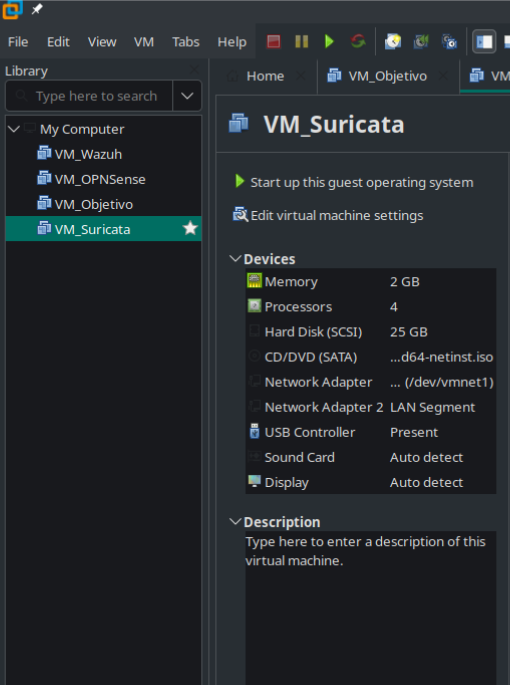
\includegraphics[scale=0.5]{tablas-images/pmv/VMware.png}
	\caption{Evidencia de creación de máquinas virtuales en el hipervisor VMware}\label{fig:vmWare}
\end{figure}

Con el propósito de garantizar que las actividades de análisis y pruebas controladas no representaran un riesgo para la infraestructura 
real, se procedió a la configuración de cuatro interfaces virtuales dentro del hipervisor VMware. Cada interfaz fue definida con un 
propósito específico: \textit{vmnet0} (WAN) configurada en modo \textit{Bridge}, \textit{vmnet1} (LAN) en modo \textit{Host-Only}, 
\textit{vmnet2} (SERVERS) igualmente en modo \textit{Host-Only} y \textit{vmnet3} (Mirror) configurada mediante un \textit{LAN Segment}. 
Esta disposición permitió establecer un entorno segmentado y controlado para el despliegue de la arquitectura de defensa en profundidad.

Asimismo, se deshabilitó el servicio DHCP nativo del hipervisor con el propósito de evitar asignaciones dinámicas de direcciones IP y 
mantener un control centralizado sobre el direccionamiento de red implementado dentro del laboratorio virtual. En este contexto, las 
interfaces \textit{vmnet1} y \textit{vmnet2} fueron configuradas con las subredes 172.16.0.0/28 y 10.0.0.0/28, respectivamente, 
permitiendo una segmentación lógica de la red y una capacidad máxima de 14 hosts por segmento. Esta decisión fue adoptada considerando las 
necesidades actuales del entorno y la posibilidad de crecimiento futuro tanto en la red de gestión como en el segmento de servidores.

Por otra parte, la interfaz \textit{vmnet3} fue configurada como un \textit{LAN Segment} dedicado al mecanismo de \textit{Port Mirroring}, 
el cual sería utilizado posteriormente para la duplicación y análisis del tráfico de red mediante el sensor \IDPS\ Suricata. Esta 
configuración permitió desacoplar el monitoreo del flujo principal de producción, evitando impactos sobre el rendimiento de la 
infraestructura virtualizada.

Es importante destacar que durante esta fase de aprovisionamiento inicial se materializa operativamente el control A.5.31 de la norma 
\ISO/IEC 27001:2022, relacionado con el establecimiento de entornos seguros y segmentados mediante mecanismos de aislamiento lógico y 
virtualización. La distribución e interconexión de las interfaces virtuales implementadas se presentan gráficamente en la 
Figura~\ref{fig:topografia}.

\begin{figure}[H]
	\centering
	\includegraphics[scale=0.5]{tablas-images/pmv/topografia.png}
	\caption{Topografía de la red implementada en el laboratorio virtualizado}\label{fig:topografia}
\end{figure}

\noindent
\subsection{Despliegue y Configuración del Firewall perimetral: OpnSense}
\noindent

Una vez consolidada la infraestructura base dentro del hipervisor, se procedió con la integración del firewall perimetral como primera 
capa de protección de la arquitectura de defensa en profundidad propuesta. Para este propósito, se seleccionó OpnSense como sistema 
operativo especializado para funciones de firewall y enrutamiento, actuando como el componente central encargado de la interconexión, 
segmentación y control del tráfico entre las diferentes zonas de confianza del laboratorio virtual~\cite{OpnsenseManual2026}.

Durante el proceso de despliegue inicial, el sistema detectó las cuatro interfaces de red virtuales suministradas por VMware. La interfaz 
\textit{em0} fue asignada al segmento WAN en modo \textit{Bridge}, permitiendo simular la conexión hacia redes externas. Por otra parte, 
las interfaces internas fueron configuradas de forma estática utilizando máscara de red “/28”, optimizando el direccionamiento y 
segmentación de la infraestructura implementada.

En este contexto, la interfaz \textit{em1} correspondiente al segmento LAN de gestión fue configurada con la dirección 172.16.0.1/28, 
mientras que la interfaz \textit{em2}, asociada al segmento SERVERS de producción, fue establecida con la dirección 10.0.0.1/28. Ambas 
interfaces operan como puertas de enlace predeterminadas para sus respectivos segmentos de red, siendo LAN que se muestra en la 
Figura~\ref{fig:fig3}, SERVERS que se muestra en la Figura~\ref{fig:fig4} y WAN que se muestra en la Figura~\ref{fig:fig5}. Permitiendo el 
control y administración centralizada del tráfico dentro de la arquitectura propuesta.

Asimismo, esta fase contribuye operativamente al cumplimiento del control A.8.22 de la norma ISO/IEC 27001:2022 y del control CLD.12.4.5 de 
la ISO/IEC 27017:2015, relacionados con la segmentación lógica de redes, separación de entornos y monitoreo del tráfico dentro de 
infraestructuras de computación en la nube.

\begin{figure}[H]
	\centering
	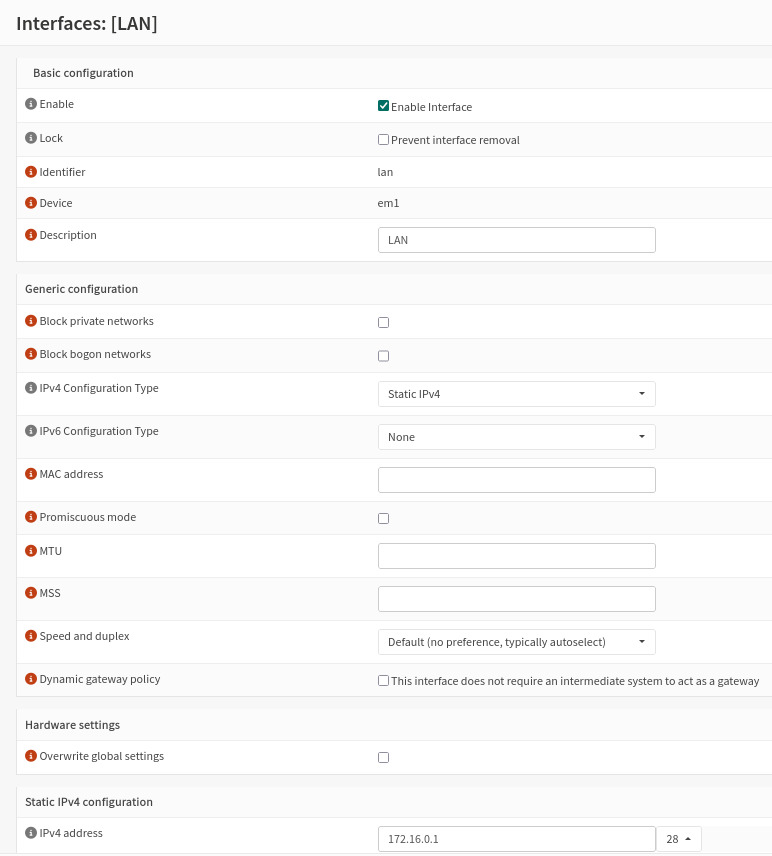
\includegraphics[scale=0.4]{tablas-images/pmv/fig3.jpeg}
	\caption{Interfaz LAN de OpnSense}\label{fig:fig3}
\end{figure}

\begin{figure}[H]
	\centering
	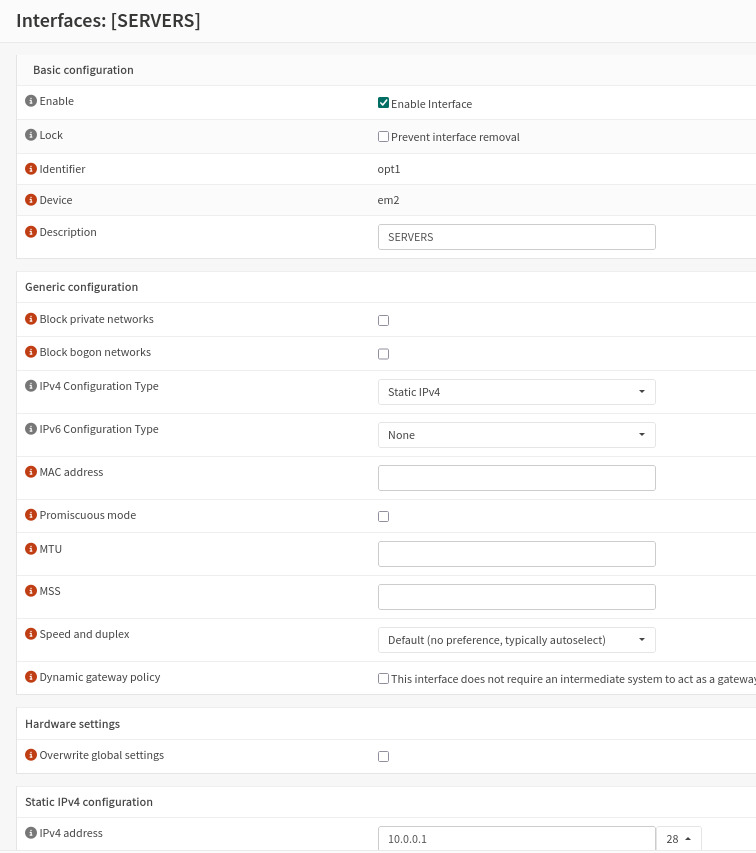
\includegraphics[scale=0.4]{tablas-images/pmv/fig4.jpeg}
	\caption{Interfaz Servers de OpnSense}\label{fig:fig4}
\end{figure}

\begin{figure}[H]
	\centering
	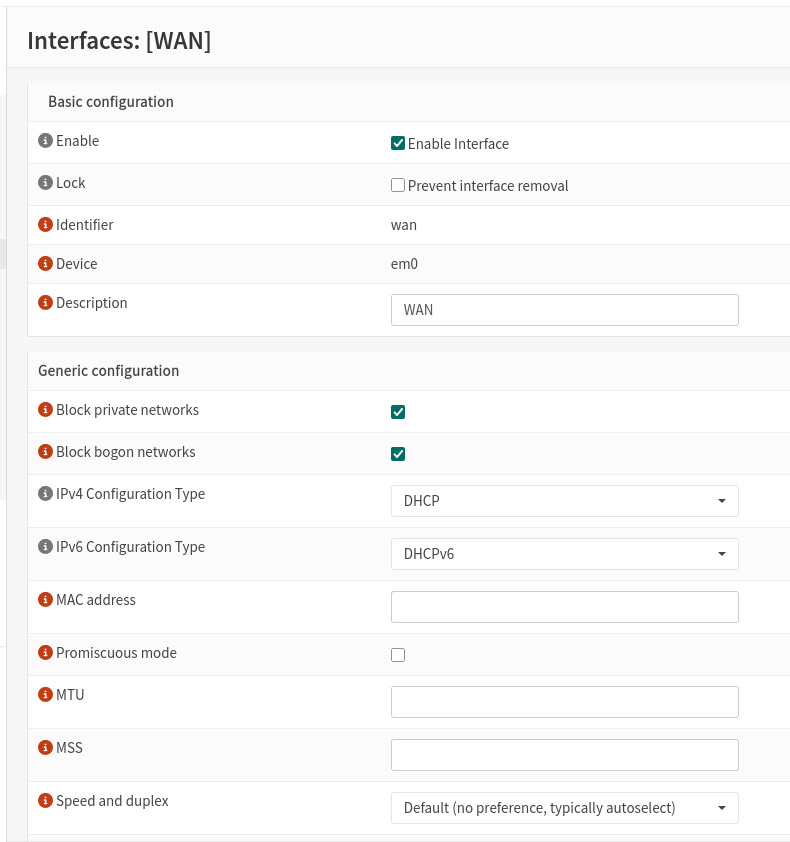
\includegraphics[scale=0.4]{tablas-images/pmv/fig5.jpeg}
	\caption{Interfaz WAN de OpnSense}\label{fig:fig5}
\end{figure}

Con el propósito de garantizar el aislamiento y control del entorno virtualizado, se habilitó el servicio DHCP nativo de OPNsense, 
configurándolo estrictamente de acuerdo con las necesidades operativas del laboratorio. En este contexto, para la interfaz \textit{em1} 
correspondiente al segmento LAN de gestión, se definió el rango de direcciones IP desde 172.16.0.2 hasta 172.16.0.14, mientras que para la 
interfaz \textit{em2} asociada al segmento SERVERS de producción, se configuró el rango comprendido entre 10.0.0.2 y 10.0.0.14.

Adicionalmente, la matriz de seguridad del firewall fue establecida bajo una política implícita de denegación total (\textit{Default Deny}), 
permitiendo únicamente el tráfico estrictamente necesario para el funcionamiento y actualización de los componentes desplegados dentro del 
laboratorio virtual. A partir de esta política, se definieron reglas específicas para autorizar exclusivamente tráfico saliente esencial 
hacia la WAN, particularmente servicios HTTP, HTTPS y DNS, necesarios para procesos de actualización y conectividad controlada.

De igual manera, se restringió de forma estricta cualquier comunicación o enrutamiento no autorizado entre el segmento de producción 
(\textit{em2}), la red de gestión (\textit{em1}) y el sistema anfitrión físico, fortaleciendo así la segmentación lógica y el aislamiento 
operativo de la infraestructura implementada. La distribución de direccionamiento IP se evidencia en la Figura~\ref{fig:fig6} y la 
configuración del servicio DHCP se presenta en la Figura~\ref{fig:fig7}.

Asimismo, esta etapa contribuye operativamente al cumplimiento del control A.8.22 de la norma ISO/IEC 27001:2022 y del control CLD.12.4.5 
de la ISO/IEC 27017:2015, relacionados con segmentación de redes, control de comunicaciones y monitoreo del tráfico dentro de 
infraestructuras de computación en la nube.

\subsubsection{Evidencia de configuración de la interfaz bridge0 y la mirror}

\begin{figure}[H]
	\centering
	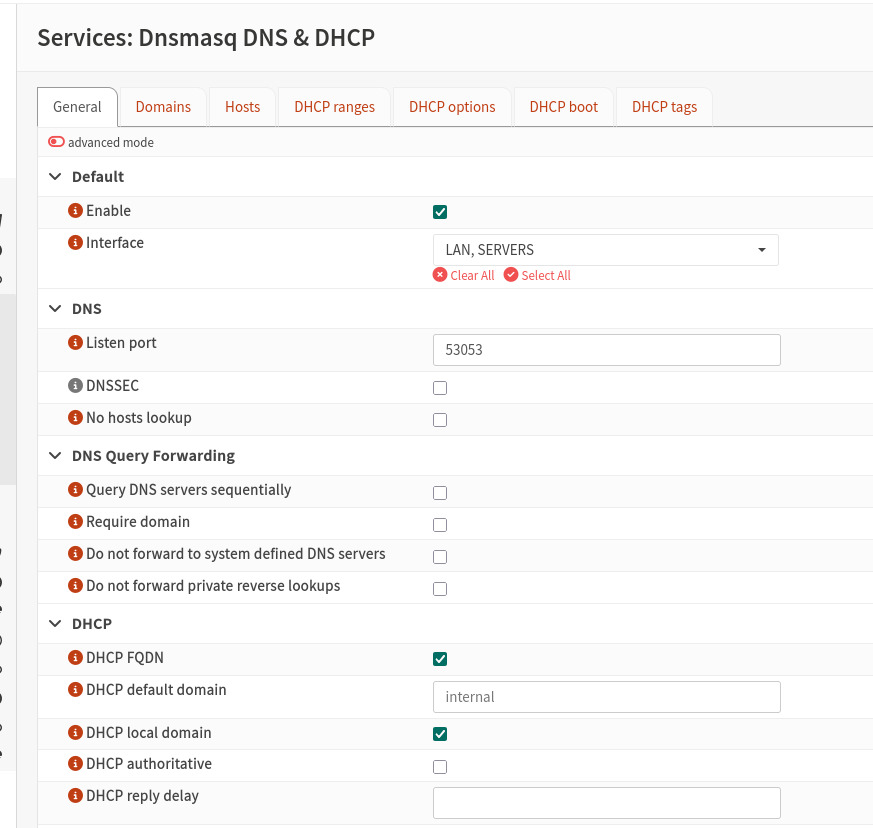
\includegraphics[scale=0.3]{tablas-images/pmv/fig6.jpeg}
	\caption{Rango de IP por segmento de red}\label{fig:fig6}
\end{figure}

\begin{figure}[H]
	\centering
	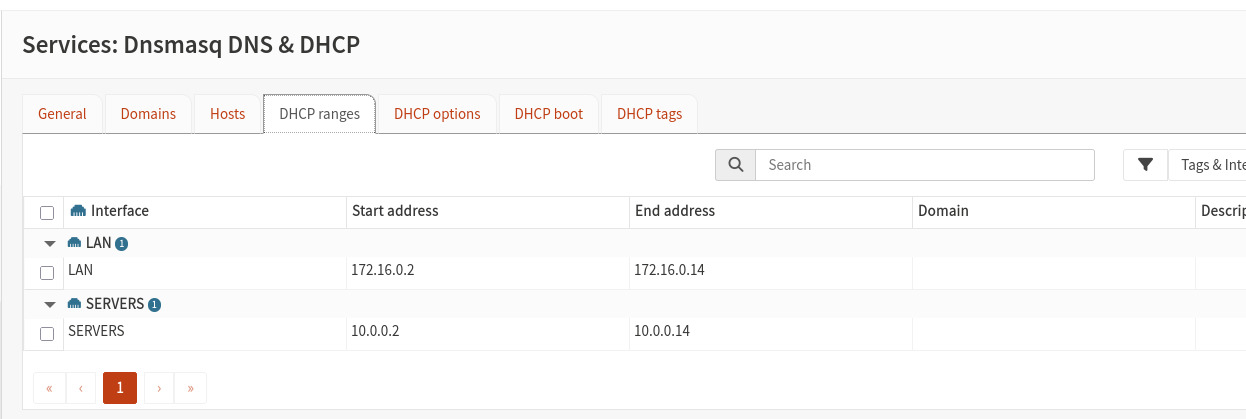
\includegraphics[scale=0.3]{tablas-images/pmv/fig7.jpeg}
	\caption{Configuración DHCP}\label{fig:fig7}
\end{figure}

Una vez configurado satisfactoriamente el servicio DHCP, se procedió con la definición de las reglas de filtrado del firewall, encargadas 
de determinar el tratamiento del tráfico de red según cada interfaz implementada dentro del laboratorio virtual. Para este propósito, se 
establecieron políticas específicas para cada segmento de red creado en la arquitectura, considerando las necesidades de conectividad, 
segmentación y supervisión del entorno.

Durante este proceso, se tomaron como referencia las reglas de filtrado utilizadas dentro de la infraestructura existente basada en 
Shorewall. Sin embargo, debido a las limitaciones propias del entorno virtualizado y al carácter de prototipo funcional de la 
implementación, se optó por configurar únicamente las reglas esenciales necesarias para garantizar conectividad controlada, 
segmentación lógica y capacidades básicas de monitoreo y filtrado dentro del laboratorio virtual.

La Figura~\ref{fig:fig8} presenta las reglas configuradas para cada una de las interfaces de red implementadas. En particular, la interfaz 
asociada al segmento \textit{Bridge} fue configurada con una regla orientada a permitir tráfico IPv4 desde cualquier origen hacia cualquier 
destino, independientemente del puerto o \textit{gateway} utilizado. Esta configuración se estableció debido a que dicha interfaz es la 
encargada de transportar el tráfico duplicado proveniente del mecanismo de \textit{Port Mirroring} hacia la máquina virtual correspondiente 
al sensor \IDPS, permitiendo el análisis e inspección del tráfico por parte de Suricata sin interferir directamente en el flujo principal 
de producción.

Asimismo, esta etapa contribuye operativamente al cumplimiento del control A.8.22 de la norma \ISO/IEC 27001:2022 y del control CLD.12.4.5 
de la \ISO/IEC 27017:2015, relacionados con control de comunicaciones, segmentación lógica y monitoreo del tráfico dentro de 
infraestructuras de computación en la nube.

\begin{figure}[H]
	\centering
	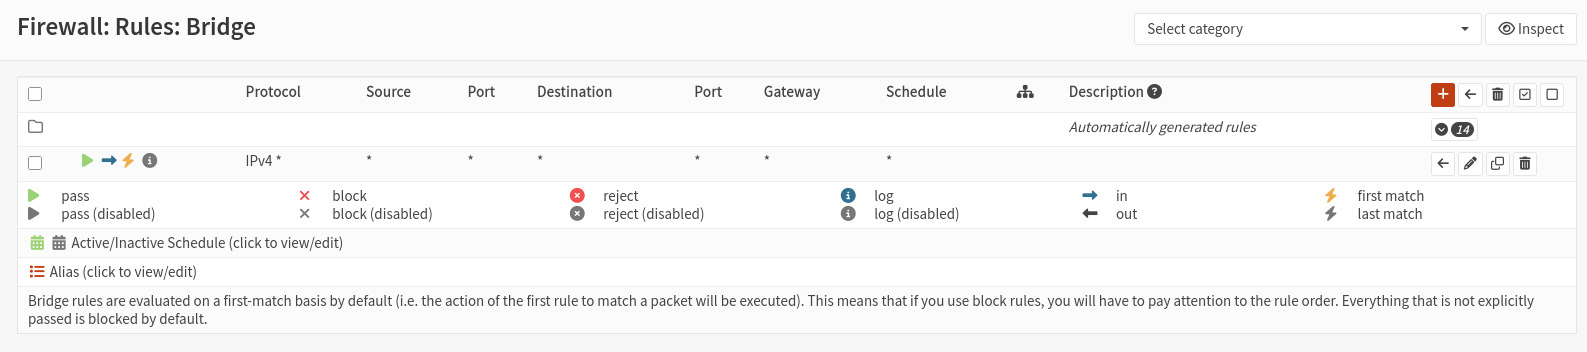
\includegraphics[scale=0.3]{tablas-images/pmv/fig8.jpeg}
	\caption{Reglas de firewall interfaz Bridge0}\label{fig:fig8}
\end{figure}

En la Figura~\ref{fig:fig9} se presentan las reglas configuradas para la interfaz LAN, las cuales permiten el tránsito de tráfico desde el 
segmento de gestión hacia los diferentes destinos requeridos dentro del entorno virtualizado. Estas reglas fueron definidas para habilitar 
conectividad controlada tanto sobre el protocolo IPv4 como IPv6, permitiendo la comunicación necesaria para tareas de administración, 
actualización y supervisión de los componentes desplegados en la arquitectura.

\begin{figure}[H]
	\centering
	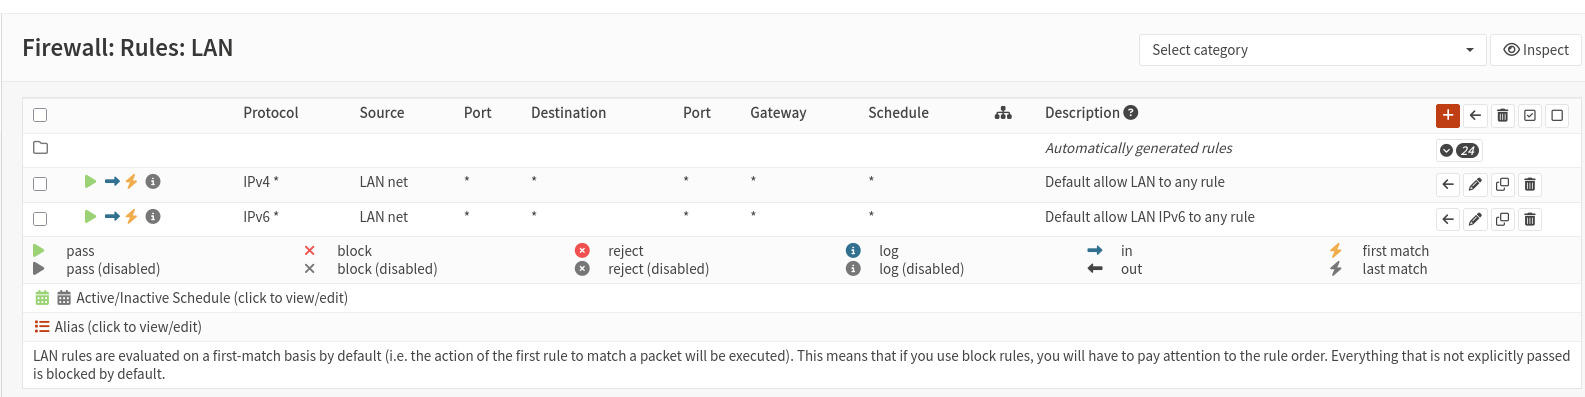
\includegraphics[scale=0.3]{tablas-images/pmv/fig9.jpeg}
	\caption{Reglas de firewall interfaz LAN}\label{fig:fig9}
\end{figure}

La interfaz \textit{Mirror} fue configurada como el punto de interconexión entre el firewall OpnSense y la máquina virtual destinada al 
análisis de tráfico mediante el sensor \IDPS. Esta interfaz opera en modo promiscuo, permitiendo la recepción y captura del tráfico 
duplicado proveniente del mecanismo de \textit{Port Mirroring} implementado dentro de la arquitectura.

Debido a la naturaleza de esta interfaz y a su función orientada exclusivamente al monitoreo y análisis de tráfico, no fue necesario 
asignarle direccionamiento IP.\@ Sin embargo, se configuraron reglas de filtrado orientadas a permitir el tránsito de tráfico IPv4 desde 
cualquier origen hacia cualquier destino, independientemente del puerto utilizado. Esta configuración garantiza la transferencia completa 
del tráfico duplicado hacia el sensor de inspección sin interferir con el flujo principal de comunicación de la infraestructura. La 
configuración descrita se presenta en la Figura~\ref{fig:fig10}.

\begin{figure}[H]
	\centering
	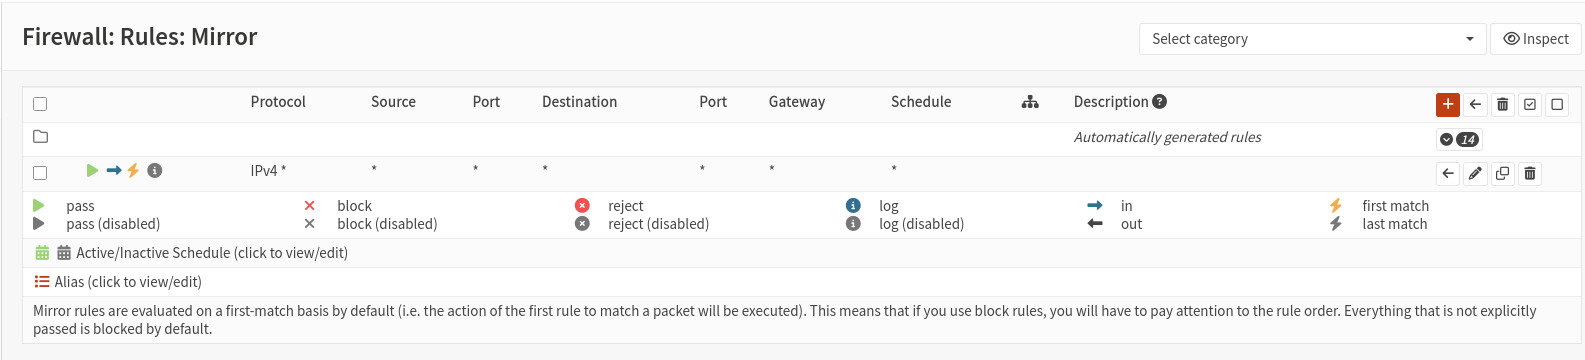
\includegraphics[scale=0.3]{tablas-images/pmv/fig10.jpeg}
	\caption{Reglas de firewall interfaz Mirror}\label{fig:fig10}
\end{figure}

La interfaz \textit{SERVERS} fue configurada de manera similar a la interfaz LAN, permitiendo el tránsito controlado de tráfico desde el 
segmento de producción hacia los destinos requeridos dentro del entorno virtualizado. Para ello, se definieron reglas orientadas a 
habilitar la comunicación mediante el protocolo IPv4, garantizando la conectividad necesaria para el funcionamiento de los servicios y 
componentes desplegados en el segmento de servidores. La configuración correspondiente se presenta en la Figura~\ref{fig:fig11}.

\begin{figure}[H]
	\centering
	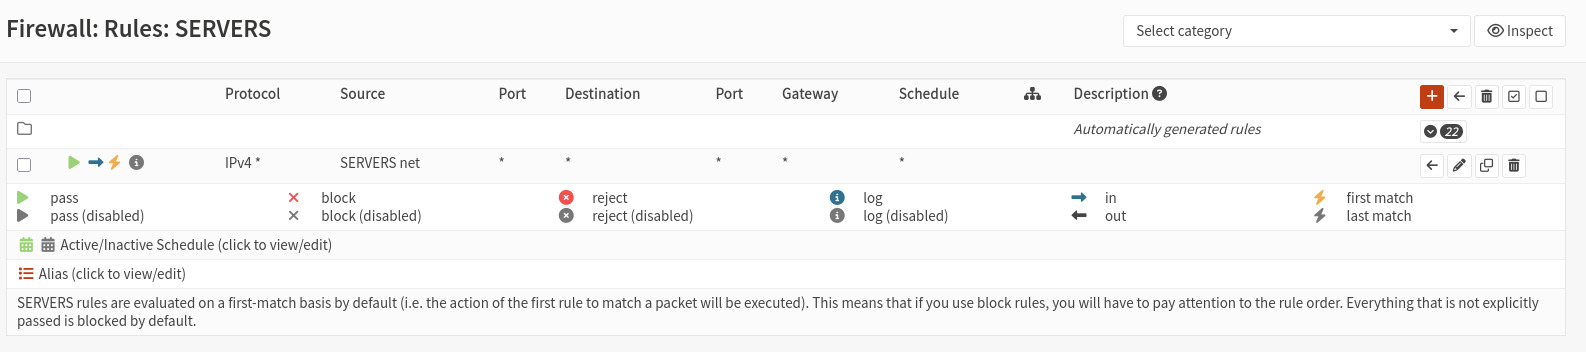
\includegraphics[scale=0.3]{tablas-images/pmv/fig11.jpeg}
	\caption{Reglas de firewall interfaz SERVER}\label{fig:fig11}
\end{figure}

Por último, la interfaz \textit{WAN} fue configurada como el punto de conexión hacia redes externas dentro del laboratorio virtual. Sobre 
esta interfaz no se definieron reglas de acceso explícitas, debido a que OpnSense aplica de manera predeterminada una política de 
denegación total (\textit{Default Deny}), bloqueando cualquier intento de comunicación no autorizado, incluyendo tráfico asociado a 
protocolos como ICMP.\@

No obstante, la interfaz mantiene habilitada la conectividad controlada hacia Internet, permitiendo únicamente el tráfico saliente 
requerido para procesos de actualización y comunicación de los componentes implementados dentro de la arquitectura. La configuración y 
comportamiento de la interfaz WAN se presentan en la Figura~\ref{fig:fig12}.

\begin{figure}[H]
	\centering
	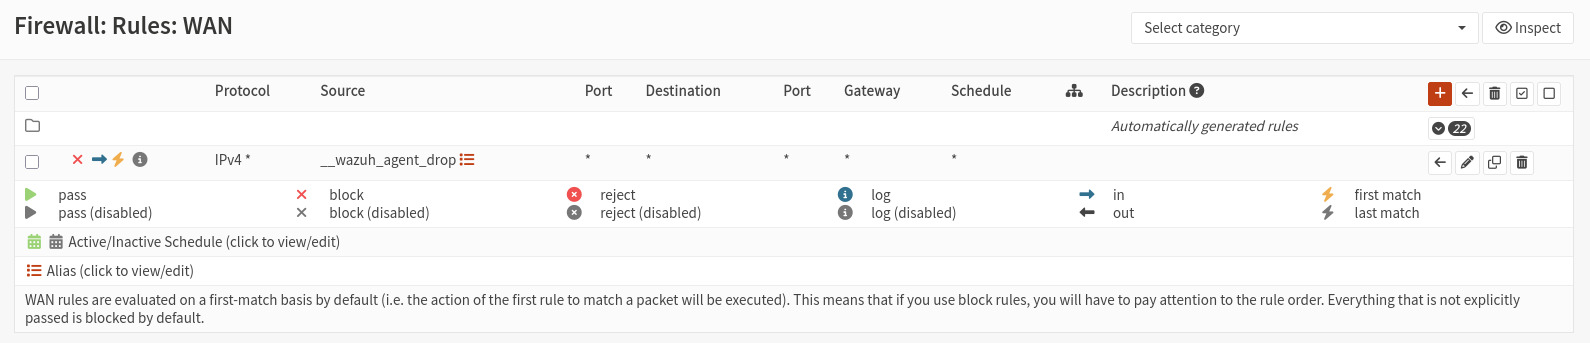
\includegraphics[scale=0.3]{tablas-images/pmv/fig12.jpeg}
	\caption{Reglas de firewall interfaz WAN}\label{fig:fig12}
\end{figure}

Es importante destacar que, sobre el sistema anfitrión, fue necesario realizar ajustes en las interfaces virtuales con el propósito de 
habilitar capacidades de conectividad y validación de tráfico dentro del laboratorio virtual. Estas modificaciones fueron aplicadas 
específicamente sobre las interfaces \textit{vmnet1} y \textit{vmnet2}, permitiendo ejecutar pruebas de conectividad, como solicitudes 
ICMP (\textit{ping}), y verificar el correcto tránsito de tráfico entre los diferentes segmentos de red implementados en la arquitectura.

La serie de comandos utilizados para realizar esta configuración se presenta a continuación.

\begin{lstlisting}[language=bash, caption={Configuración de interfaces virtuales mediante NetworkManager}, label={lst:nmcli}]
	
nmcli connection modify vmnet1 ipv4.method auto &&
nmcli connection modify vmnet2 ipv4.method auto

nmcli connection up vmnet1
nmcli connection up vmnet2

\end{lstlisting}

El primer comando permite configurar la interfaz de red para obtener automáticamente una dirección IP mediante el servicio DHCP 
administrado por OpnSense, mientras que el segundo comando habilita y reinicia la interfaz virtual correspondiente, asegurando la 
aplicación inmediata de la configuración realizada dentro del sistema anfitrión.

Posteriormente, para habilitar capacidades de auditoría pasiva y monitoreo de tráfico, fue necesario resolver las limitaciones nativas de 
VMware Workstation relacionadas con el manejo de interfaces en modo promiscuo. Para ello, se implementó un puente lógico (\textit{Bridge}) 
dentro de OpnSense, utilizando la interfaz \textit{em3} configurada sin direccionamiento IP y operando en modo promiscuo mediante el uso 
del segmento virtual \textit{LAN Segment} proporcionado por VMware.

Esta configuración permitió clonar de manera asíncrona el tráfico que transita por la red LAN y redirigirlo hacia el puerto espejo 
(\textit{SPAN Segment}), donde el sensor \IDPS\ permanece en estado de escucha para realizar tareas de inspección y análisis profundo del 
tráfico. De esta manera, el monitoreo puede ejecutarse sin interferir directamente sobre el flujo principal de producción del entorno 
virtualizado.

Con este despliegue se materializan operativamente el control A.8.22 de la norma ISO/IEC 27001:2022, relacionado con la segregación y 
segmentación de redes, y el control CLD.12.4.5 de la ISO/IEC 27017:2015, asociado al monitoreo y supervisión del tráfico dentro de 
infraestructuras de computación en la nube. El comando utilizado para resolver las restricciones de permisos impuestas por VMware durante 
la configuración de interfaces en modo promiscuo se presenta a continuación.

\begin{lstlisting}[language=bash, caption={Asignación de permisos sobre interfaces virtuales de VMware}, label={lst:vmware_permissions}]
	
	sudo chown root:$USER /dev/vmnet*
	sudo chmod 0660 /dev/vmnet*

\end{lstlisting}

En la Figura~\ref{fig:fig13} se presenta la configuración realizada para la implementación del mecanismo de \textit{Port Mirroring}, así 
como la definición de la interfaz encargada de recibir la copia del tráfico que transita por el puente lógico \textit{Bridge0} de OpnSense. 
Este puente fue configurado integrando las interfaces correspondientes a los segmentos LAN y SERVERS, permitiendo supervisar el tráfico de 
entrada y salida, así como la comunicación entre máquinas pertenecientes al mismo segmento y entre diferentes segmentos de red.

La interfaz WAN no fue incluida dentro del mecanismo de replicación de tráfico debido a la alta cantidad de tráfico externo no relevante, 
lo cual podría generar saturación en el canal de análisis del sensor \IDPS\ y afectar el rendimiento de los procesos de inspección y 
detección de amenazas.

Asimismo, la interfaz \textit{Bridge0}, que se muestra en la Figura~\ref{fig:fig14}, actúa de manera similar a un switch virtual, 
permitiendo capturar el tráfico que circula entre las interfaces integradas y generar una copia destinada a la interfaz \textit{em3}, 
configurada como puerto SPAN dentro del mecanismo de monitoreo. Debido a su funcionamiento interno, no fue necesario configurar el puente 
en modo promiscuo, ya que la replicación del tráfico se realiza de forma nativa dentro del entorno virtualizado. La configuración 
correspondiente al puente lógico, se evidencia en la Figura~\ref{fig:fig15}.

\begin{figure}[H]
	\centering
	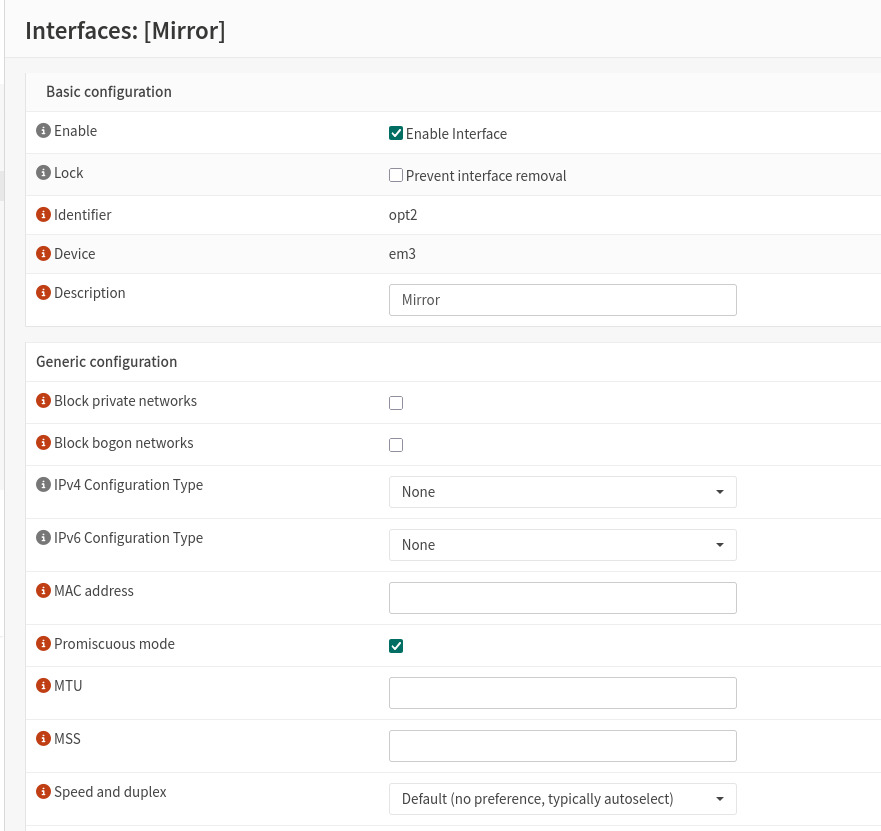
\includegraphics[scale=0.3]{tablas-images/pmv/fig13.jpeg}
	\caption{Configuración de la interfaz Mirror}\label{fig:fig13}
\end{figure}

\begin{figure}[H]
	\centering
	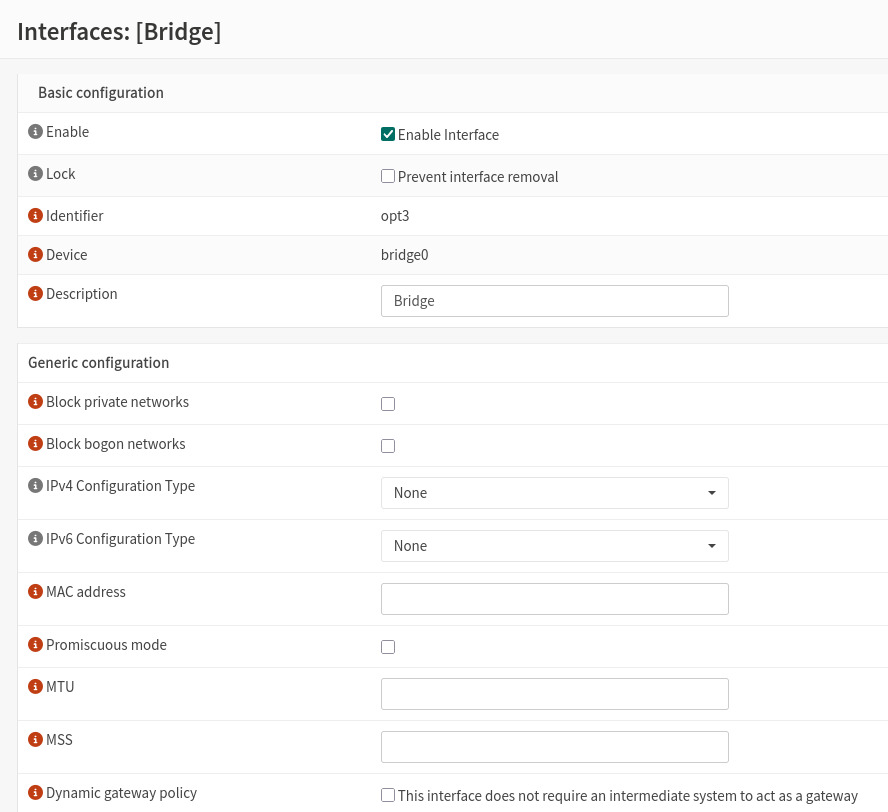
\includegraphics[scale=0.3]{tablas-images/pmv/fig14.jpeg}
	\caption{Configuración de la interfaz Bridge0}\label{fig:fig14}
\end{figure}

\begin{figure}[H]
	\centering
	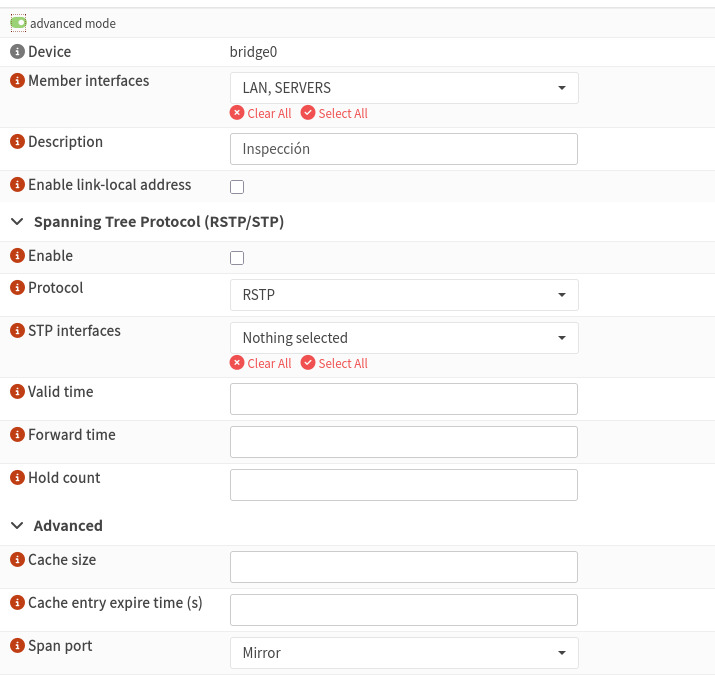
\includegraphics[scale=0.3]{tablas-images/pmv/fig15.jpeg}
	\caption{Edición de la interfaz Bridge0}\label{fig:fig15}
\end{figure}

\subsection{Inspección profunda y detección de amenazas: IDPS Suricata}
\noindent

En este apartado se continúa con la implementación de la segunda capa de la arquitectura de defensa en profundidad, enfocada en la 
auditoría y supervisión del tráfico interno mediante el despliegue del Sistema de Detección y Prevención de Intrusiones (\IDPS) 
Suricata~\cite{SuricataGuide2025}, implementado sobre un sistema operativo Debian 13 en modo CLI.\@ El objetivo principal de este 
componente consiste en realizar procesos de inspección profunda de paquetes (\textit{Deep Packet Inspection}, DPI) sobre el tráfico 
clonado proveniente del firewall OpnSense, permitiendo identificar anomalías, eventos sospechosos y posibles patrones de ataque dirigidos 
a la infraestructura tecnológica.

Una vez preparado el entorno virtual y establecida la conectividad mediante las interfaces administradas por OPNsense, se procedió con el 
acceso a la máquina virtual destinada al \IDPS\ para realizar la instalación nativa del motor de detección y su posterior configuración 
estructural dentro del laboratorio virtual. Los comandos utilizados para este proceso se presentan a continuación.

\begin{lstlisting}[language=bash, caption={Instalación del motor IDPS Suricata en Debian 13}, label={lst:suricata_install}]

sudo apt update && sudo apt install suricata -y

\end{lstlisting}

Una vez instalada la herramienta, se procedió con la modificación del archivo principal de configuración de Suricata denominado 
\textit{suricata.yaml}, ubicado en la ruta \texttt{/etc/suricata/suricata.yaml}. Dentro de este archivo se ajustaron parámetros 
fundamentales para el funcionamiento del \IDPS\ dentro del laboratorio virtual, este archivo se muestra en la Figura~\ref{fig:fig16}.

Entre las configuraciones realizadas, se definió la variable \texttt{\$HOME\_NET}, utilizada para especificar los segmentos de red 
internos implementados en la arquitectura propuesta. Asimismo, dentro de la sección \textit{AF\_PACKET}, evidenciado en la 
Figura~\ref{fig:fig17}, se configuró la interfaz encargada de recibir el tráfico clonado proveniente del firewall OPNsense mediante el 
mecanismo de \textit{Port Mirroring}. Para este propósito, se utilizó la interfaz \texttt{ens36}, correspondiente al segmento SPAN 
destinado al análisis pasivo del tráfico en modo promiscuo.


\begin{figure}[H]
	\centering
	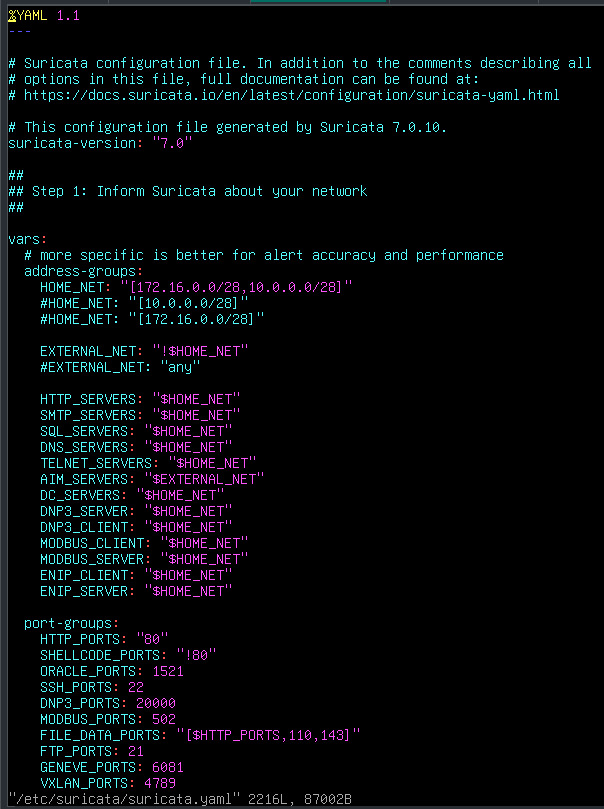
\includegraphics[scale=0.3]{tablas-images/pmv/fig16.jpeg}
	\caption{Archivo yaml de Suricata}\label{fig:fig16}
\end{figure}

\begin{figure}[H]
	\centering
	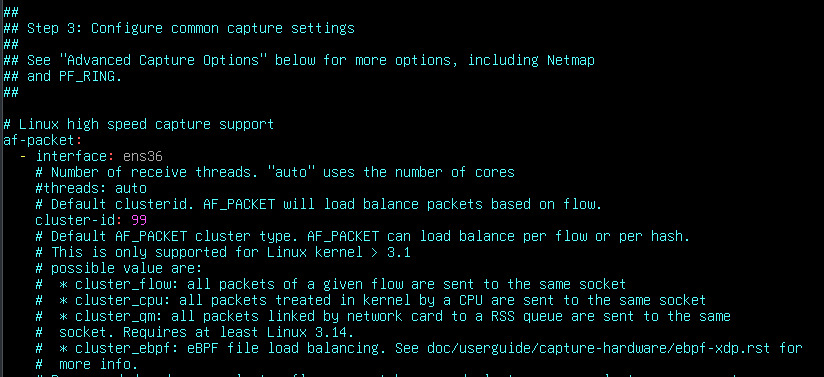
\includegraphics[scale=0.5]{tablas-images/pmv/fig17.jpeg}
	\caption{Configuración de AF\_PACKET}\label{fig:fig17}
\end{figure}

Posteriormente a la configuración realizada en el archivo \textit{suricata.yaml}, se procedió a habilitar la interfaz de red del sistema 
Debian donde se encuentra desplegado Suricata en modo promiscuo. Esta configuración permitió que la interfaz pudiera capturar y procesar 
los paquetes clonados provenientes del firewall OPNsense, incluso cuando dichos paquetes no estuvieran dirigidos específicamente a la 
dirección MAC de la máquina virtual asociada al \IDPS.

La Figura~\ref{fig:fig18} presenta el comando utilizado para habilitar el modo promiscuo, así como la verificación de la interfaz de red 
operando bajo esta configuración dentro del entorno virtualizado.

\begin{lstlisting}[language=bash, caption={Habilitación del modo promiscuo en la interfaz de monitoreo}, label={lst:promisc}]

sudo ip link set dev ens36 promiscuous on

\end{lstlisting}

\begin{figure}[H]
	\centering
	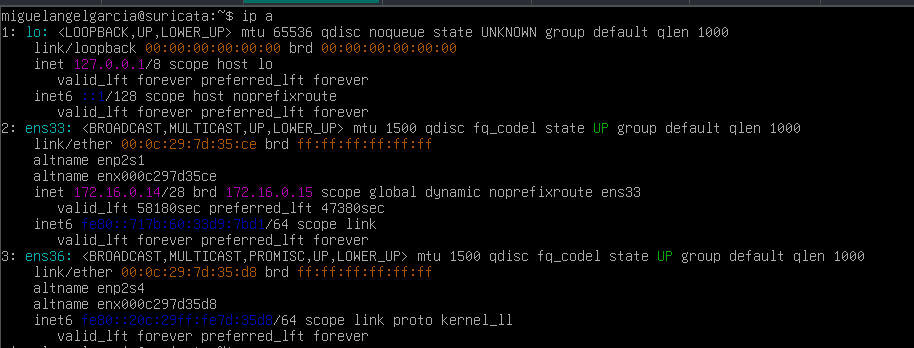
\includegraphics[scale=0.5]{tablas-images/pmv/fig18.jpeg}
	\caption{Evidencia de configuración en modo promiscuo de la interfaz ens36}\label{fig:fig18}
\end{figure}

Posteriormente a la configuración de la interfaz de monitoreo \texttt{ens36}, se procedió con la habilitación e inicio del servicio de 
Suricata, así como con la validación del archivo de configuración \textit{suricata.yaml}, con el propósito de verificar que no existieran 
errores estructurales antes de poner en funcionamiento el motor de detección dentro del laboratorio virtual.

Los comandos utilizados para habilitar, iniciar y validar el servicio de Suricata se presentan a continuación.

\begin{lstlisting}[language=bash, caption={Habilitación e inicio del servicio Suricata}, label={lst:suricata_service}]

sudo systemctl enable suricata && sudo systemctl start suricata
sudo suricata -T -c /etc/suricata/suricata.yaml -v

\end{lstlisting}

Posteriormente, la Figura~\ref{fig:fig19} presenta el estado actual del servicio una vez habilitado e iniciado correctamente dentro del 
sistema Debian implementado para el \IDPS.

\begin{figure}[H]
	\centering
	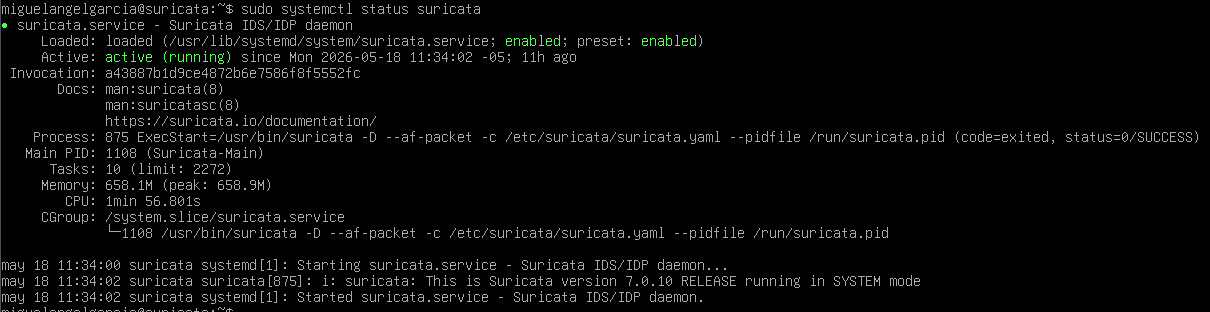
\includegraphics[scale=0.3]{tablas-images/pmv/fig19.jpeg}
	\caption{Evidencia de habilitación e inicio del servicio de suricata}\label{fig:fig19}
\end{figure}

Con el propósito de validar el correcto funcionamiento del modo promiscuo y del mecanismo de \textit{Bridge} configurado en OPNsense, se 
realizó una captura pasiva de tráfico desde la máquina virtual destinada al \IDPS. Esta prueba permitió verificar la recepción de paquetes 
provenientes de otros segmentos de red mediante tráfico ICMP generado desde el sistema anfitrión hacia OPNsense y hacia la máquina virtual 
de Suricata.

Para ello, se ejecutó un proceso de monitoreo sobre la interfaz \texttt{ens36}, encargada de recibir el tráfico clonado mediante el 
mecanismo de \textit{Port Mirroring}. La Figura~\ref{fig:fig20} presenta el análisis del tráfico capturado dentro del entorno virtualizado 
utilizando el siguiente comando.

\begin{lstlisting}[language=bash, caption={Captura pasiva de tráfico ICMP mediante tcpdump}, label={lst:tcpdump_icmp}]

	sudo tcpdump -i ens36 -n icmp

\end{lstlisting}

\begin{figure}[H]
	\centering
	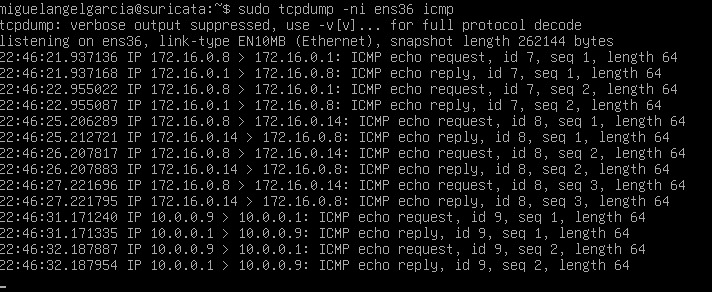
\includegraphics[scale=0.5]{tablas-images/pmv/fig20.jpeg}
	\caption{Evidencia de tráfico entre los segmentos de redes capturado}\label{fig:fig20}
\end{figure}

De igual manera, se realizó la actualización del conjunto de firmas y reglas utilizadas por Suricata, con el propósito de mantener el motor 
de detección preparado para identificar patrones asociados a actividades maliciosas, anomalías de tráfico e intentos de intrusión dentro 
de la infraestructura implementada.

Este proceso permite incorporar reglas actualizadas provenientes de repositorios abiertos y comerciales compatibles con Suricata, 
fortaleciendo así las capacidades de detección y análisis del \IDPS. El comando utilizado para la actualización de las reglas se presenta 
a continuación.

\begin{lstlisting}[language=bash, caption={Actualización de reglas y firmas de Suricata}, label={lst:suricata_update}]

	sudo suricata-update

\end{lstlisting}

Finalmente, Suricata almacena los eventos y registros generados durante el proceso de monitoreo dentro del archivo \textit{eve.json}, que 
se muestra en la Figura~\ref{fig:fig21}, ubicado en la ruta \texttt{/var/log/suricata/eve.json}. Este archivo centraliza información 
relacionada con alertas, eventos de red, tráfico analizado y actividades detectadas por el \IDPS\ dentro del entorno virtualizado.

Por otra parte, las reglas utilizadas por Suricata se encuentran almacenadas en el archivo \textit{suricata.rules}, localizado en la ruta 
\texttt{/var/lib/suricata/rules/suricata.rules}. Este archivo contiene el conjunto de firmas y reglas descargadas desde los repositorios 
oficiales de la comunidad de Suricata, las cuales son utilizadas para la detección de eventos y patrones asociados a amenazas de seguridad. 
Asimismo, dichas reglas pueden ser modificadas, ajustadas o ampliadas de acuerdo con las necesidades específicas del entorno o los 
requerimientos definidos por la organización.

La Figura~\ref{fig:fig22} presenta la visualización en tiempo real de los eventos generados mediante el siguiente comando.

\begin{lstlisting}[language=bash, caption={Monitoreo en tiempo real de registros en Suricata}, label={lst:evejson}]

	tail -f /var/log/suricata/eve.json

\end{lstlisting}

Posteriormente, la Figura~\ref{fig:fig23} muestra el contenido del archivo \textit{suricata.rules}, evidenciando las reglas predeterminadas 
suministradas por la comunidad de Suricata y utilizadas por el motor de detección dentro de la arquitectura implementada.

\begin{figure}[H]
	\centering
	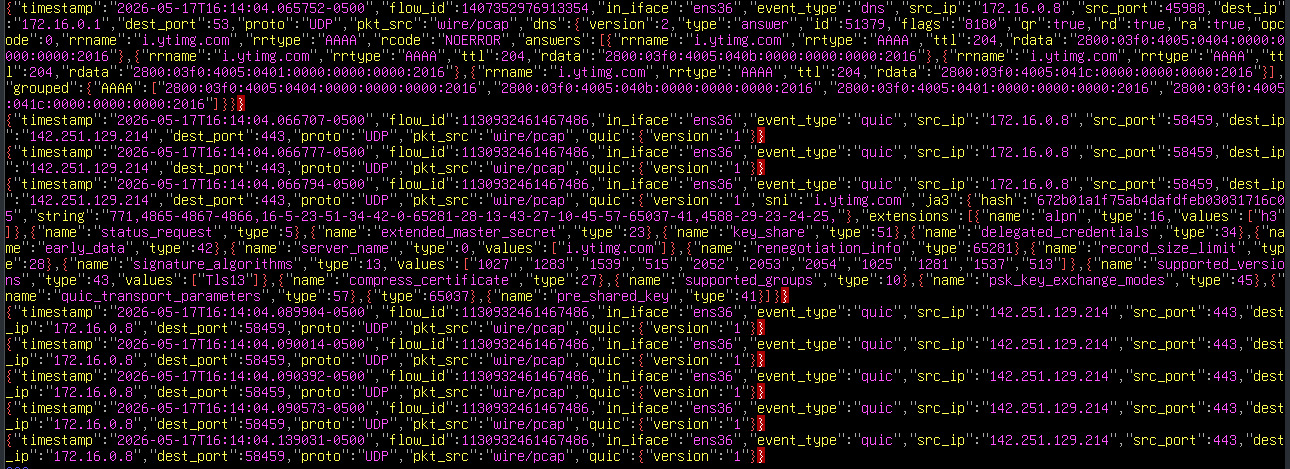
\includegraphics[scale=0.3]{tablas-images/pmv/fig21.jpeg}
	\caption{Archivo de reglas de Suricata eve.json}\label{fig:fig21}
\end{figure}

\begin{figure}[H]
	\centering
	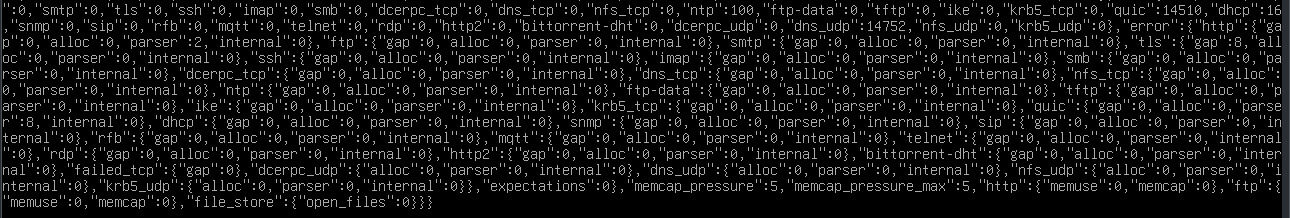
\includegraphics[scale=0.3]{tablas-images/pmv/fig22.jpeg}
	\caption{Tráfico detectado en tiempo real}\label{fig:fig22}
\end{figure}

\begin{figure}[H]
	\centering
	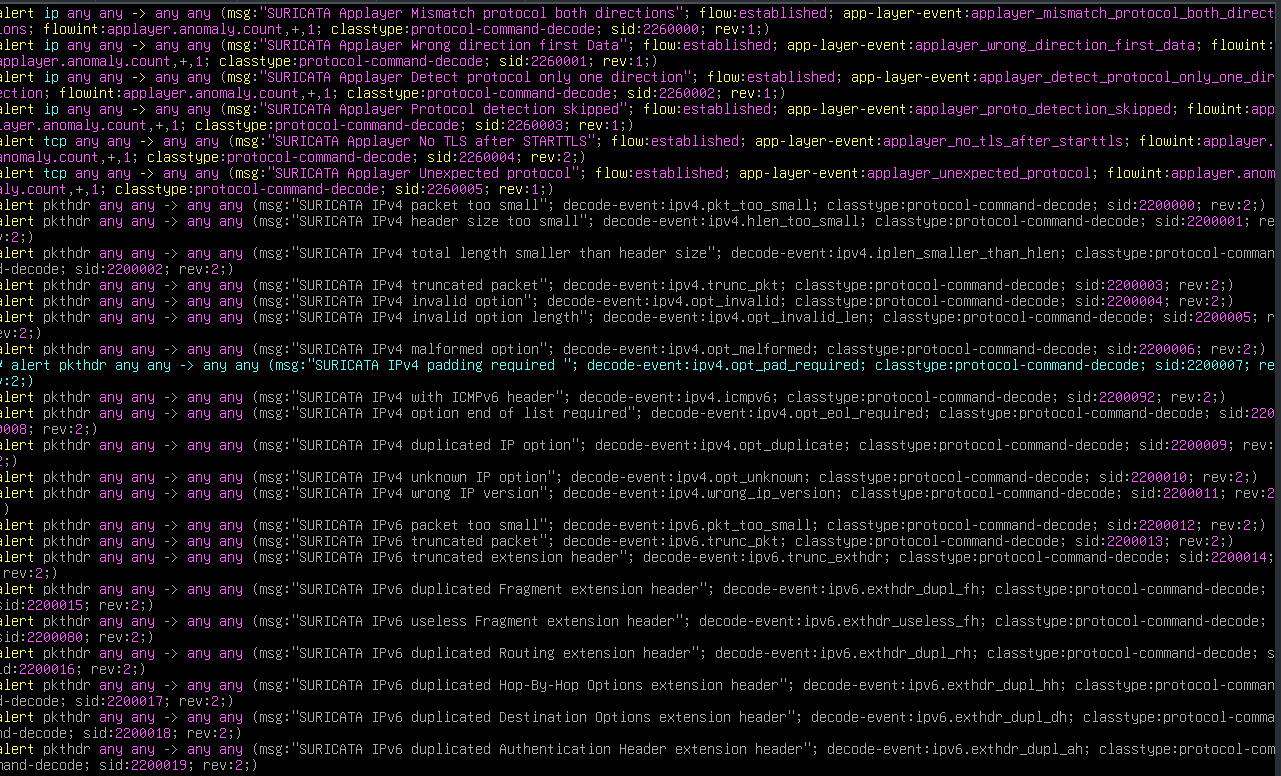
\includegraphics[scale=0.3]{tablas-images/pmv/fig23.jpeg}
	\caption{Demostración del archivo de reglas en suricata}\label{fig:fig23}
\end{figure}

Finalmente, mediante el despliegue operativo de Suricata y su configuración basada en comandos reales dentro del laboratorio virtual, fue 
posible validar las capacidades de interceptación, monitoreo y análisis del tráfico replicado a través del mecanismo de 
\textit{Port Mirroring}. Asimismo, la actualización continua del motor de detección mediante firmas de amenazas y la supervisión activa de 
los flujos de comunicación permitieron fortalecer las capacidades de auditoría y monitoreo continuo de la infraestructura implementada.

De esta manera, la integración del \IDPS\ contribuye operativamente al cumplimiento de los controles A.5.7, A.5.24 y A.8.16 de la norma 
\ISO/IEC 27001:2022, relacionados con inteligencia de amenazas, planificación y preparación para la gestión de incidentes de seguridad de 
la información, así como monitoreo y supervisión de actividades dentro de entornos tecnológicos.

\section{Centralización y gestión de eventos: SIEM Wazuh}
\noindent

La presente fase corresponde a la última capa de la arquitectura de defensa en profundidad y se consolidó mediante la implementación de la 
plataforma \SIEM\ Wazuh~\cite{WazuhDocs2026}, desplegada sobre una máquina virtual dedicada con sistema operativo Debian 13. La finalidad 
principal de este componente consiste en centralizar los registros de auditoría generados dentro del laboratorio virtual, correlacionar 
eventos de seguridad en tiempo real, fortalecer las capacidades de monitoreo continuo y proporcionar un panel unificado para la supervisión 
y gestión de incidentes de seguridad.

Para el proceso de instalación se utilizó el script oficial suministrado por la documentación de Wazuh, permitiendo mantener compatibilidad 
y alineación con los lineamientos recomendados por la plataforma. Asimismo, aunque Wazuh permite desplegar de manera independiente cada 
uno de sus componentes, en este trabajo se optó por una instalación tipo \textit{All-in-One}, la cual aprovisiona e integra de manera 
nativa los principales servicios del ecosistema Wazuh dentro de una única máquina virtual.

En este contexto, la instalación implementada incluyó los servicios \textit{Wazuh Indexer}, \textit{Wazuh Manager} y \textit{Wazuh 
Dashboard}, encargados respectivamente del almacenamiento e indexación de eventos, la administración y correlación de alertas, y la 
visualización centralizada de la información de seguridad generada dentro de la infraestructura.

Los comandos utilizados para la instalación y habilitación de los servicios de Wazuh se presentan a continuación.

\begin{lstlisting}[language=bash, caption={Instalación y activación de servicios de Wazuh}, label={lst:wazuh_install}]

curl -sO https://packages.wazuh.com/4.14/wazuh-install.sh && \
sudo bash ./wazuh-install.sh -a

sudo systemctl start wazuh-indexer
sudo systemctl start wazuh-manager.service
sudo systemctl start wazuh-dashboard.service

\end{lstlisting}

Una vez instalada la herramienta SIEM Wazuh, se proporciona un usuario y una contraseña únicos, por lo que se recomienda almacenarlos de 
forma inmediata y segura. Esto se debe a que, si posteriormente se requiere modificar dichas credenciales, pueden presentarse problemas de 
autenticación que afecten el funcionamiento óptimo de la herramienta. Asimismo, se recomienda reiniciar simultáneamente los tres servicios 
principales cada vez que se actualicen las configuraciones de los archivos correspondientes.

En la Figura~\ref{fig:fig24} se presenta el \textit{overview} de la plataforma, donde se visualizan los niveles de alerta y los 
accesos directos a las diferentes opciones disponibles en la herramienta.

\begin{figure}[H]
	\centering
	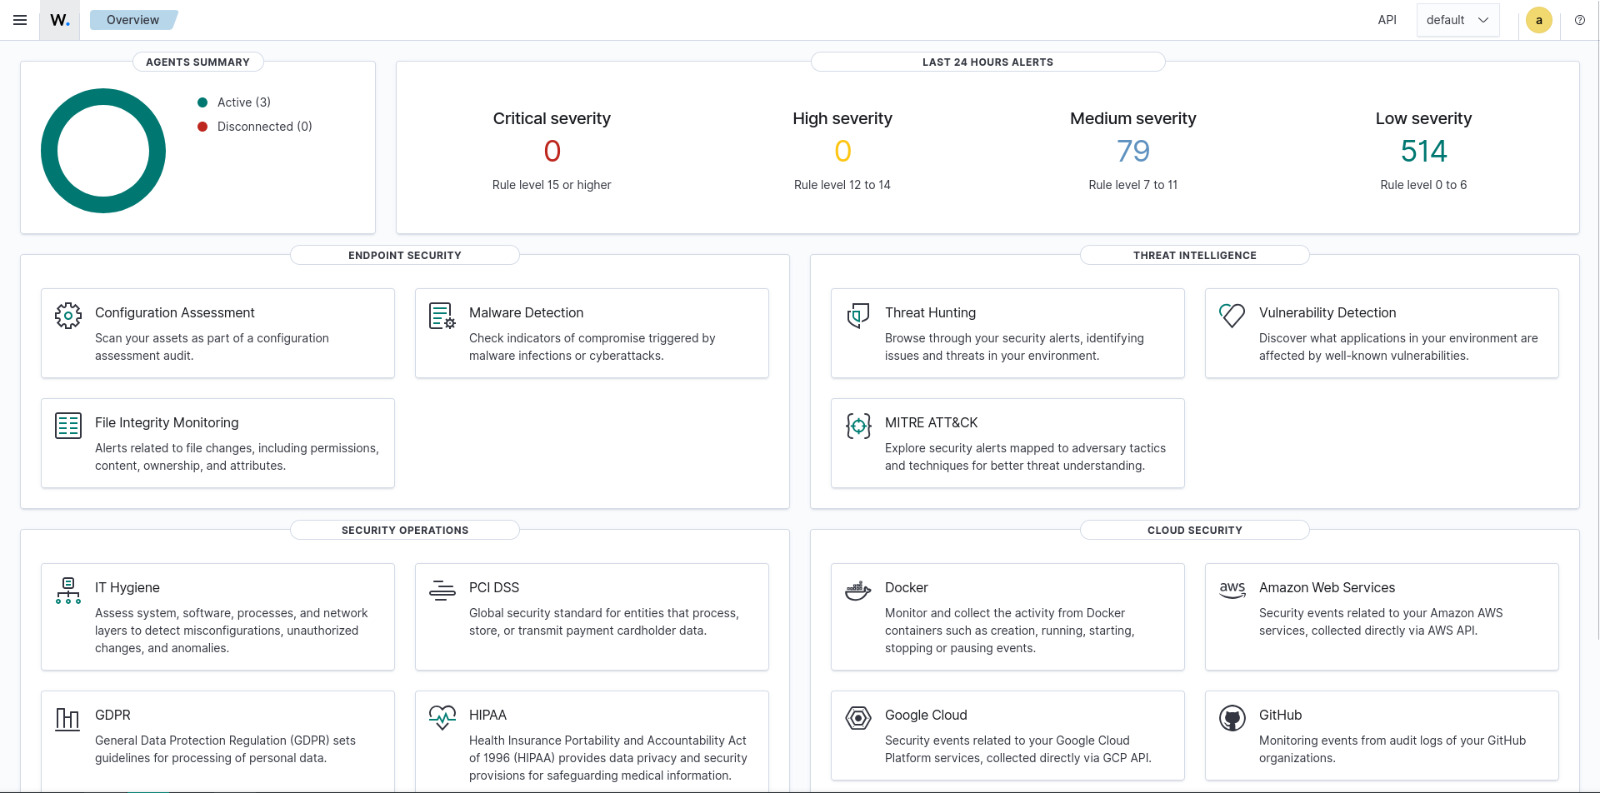
\includegraphics[scale=0.3]{tablas-images/pmv/fig24.jpeg}
	\caption{Overview principal de la herramienta SIEM Wazuh}\label{fig:fig24}
\end{figure}

Posteriormente, se continúa con uno de los componentes más importantes de Wazuh: los agentes. Estos son los encargados de recolectar 
información y registrar las actividades realizadas en los diferentes dispositivos o \textit{endpoints}, enviando posteriormente dichos 
registros al servidor Wazuh para su análisis, correlación y visualización centralizada. Los eventos generados son clasificados según 
niveles de severidad, los cuales pueden corresponder a categorías bajas, medias, altas o críticas, dependiendo del impacto identificado.

Antes de presentar el resumen de los \textit{endpoints} donde fueron desplegados los agentes de Wazuh, es importante destacar que la 
plataforma permite generar automáticamente un script de instalación personalizado según el sistema operativo del dispositivo objetivo. 
Posteriormente, se asigna un nombre al agente y se configura la dirección IP del servidor donde se encuentra alojado Wazuh. En la 
Figura~\ref{fig:fig25} se muestra la interfaz web de configuración, las opciones disponibles y el comando resultante 
para la instalación del agente Wazuh.

\begin{figure}[H]
	\centering
	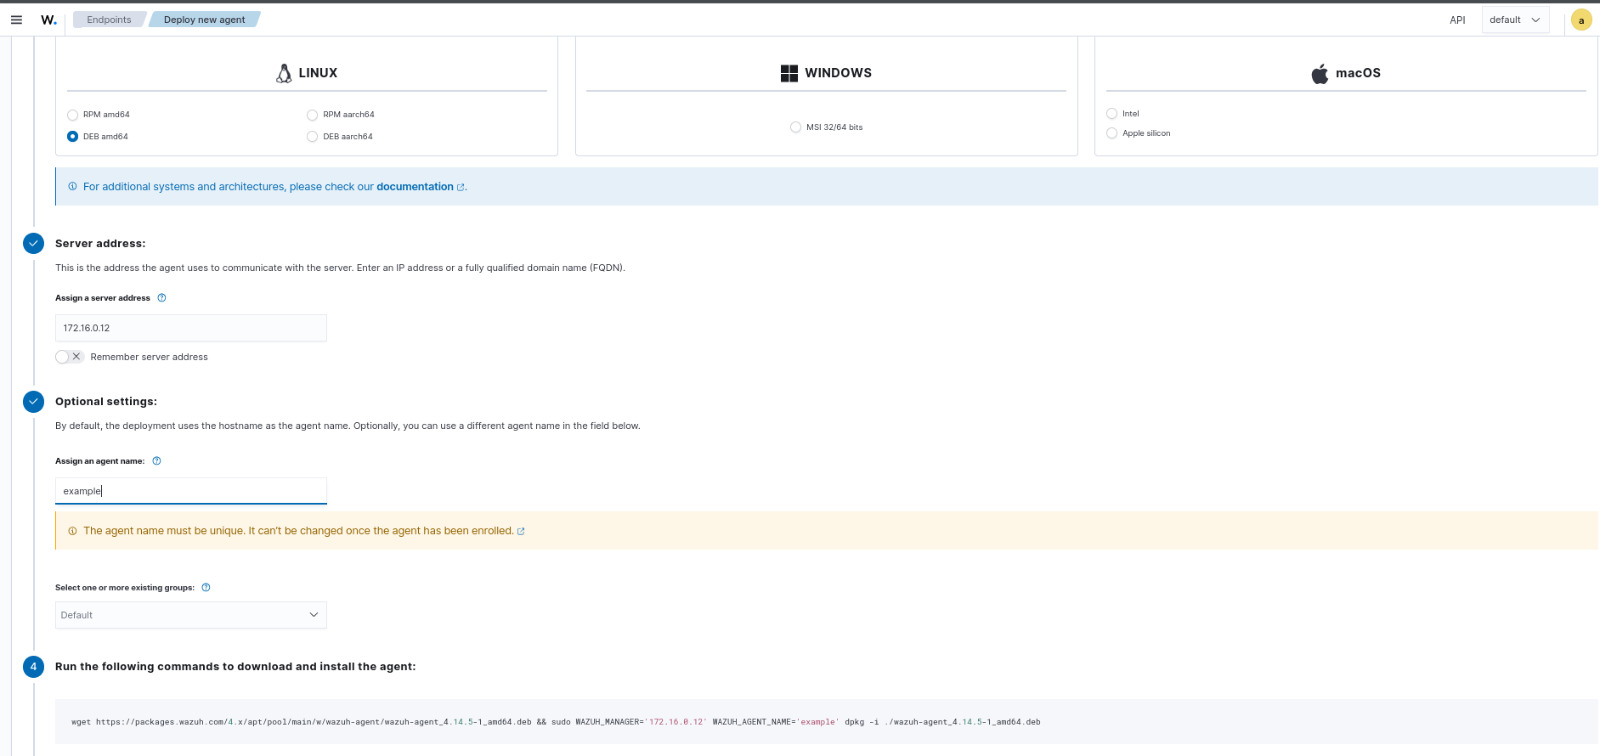
\includegraphics[scale=0.3]{tablas-images/pmv/fig25.jpeg}
	\caption{Demostración de la interfaz de creación de agentes}\label{fig:fig25}
\end{figure}

\begin{lstlisting}[language=bash, caption={Comando generado para la instalación del agente Wazuh}, label={lst:wazuh_agent_install}]

wget https://packages.wazuh.com/4.x/apt/pool/main/w/wazuh-agent/wazuh-agent_4.14.5-1_amd64.deb && sudo WAZUH_MANAGER='172.16.0.12' 
WAZUH_AGENT_NAME='Example' dpkg -i ./wazuh-agent_4.14.5-1_amd64.deb

\end{lstlisting}

En la Figura~\ref{fig:fig26} se observa la sección donde se encuentran desplegados los tres agentes actualmente 
configurados en la infraestructura: OpnSense, el sistema IDPS Suricata y la máquina objetivo.

\begin{figure}[H]
	\centering
	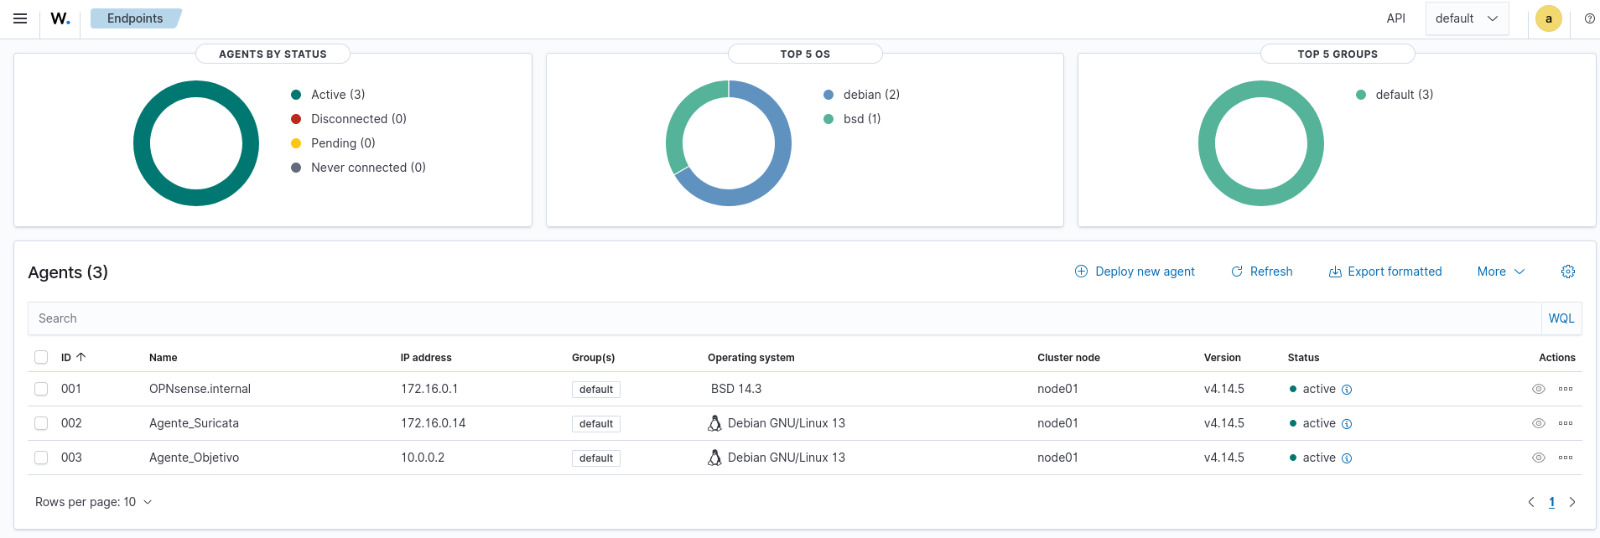
\includegraphics[scale=0.3]{tablas-images/pmv/fig26.jpeg}
	\caption{Resumen de endpoints establecidos para los agentes de Wazuh}\label{fig:fig26}
\end{figure}

Una vez instalado cada agente en su respectiva máquina, se dispone de un archivo de configuración común denominado \texttt{ossec.conf}, 
ubicado en la ruta \texttt{/var/ossec/etc/ossec.conf}. Este archivo tiene como propósito definir tanto la configuración del \textit{wazuh-
manager} como las actividades y monitoreos específicos que los agentes deben ejecutar en cada dispositivo.

En el caso de OpnSense, la instalación del agente Wazuh se realiza mediante un \textit{plugin}, por lo que únicamente es necesario 
configurarlo desde la interfaz web del sistema, quedando posteriormente habilitado como un servicio automático. Asimismo, es importante 
resaltar que el agente Wazuh debe tener acceso a los registros generados por el firewall para permitir la correcta correlación de eventos y 
el monitoreo centralizado de seguridad.

En la Figura~\ref{fig:fig27} se evidencia la disponibilidad del \textit{plugin} y en la Figura~\ref{fig:fig28} se mmuestra la 
configuración correspondiente realizada en OpnSense.

\begin{figure}[H]
	\centering
	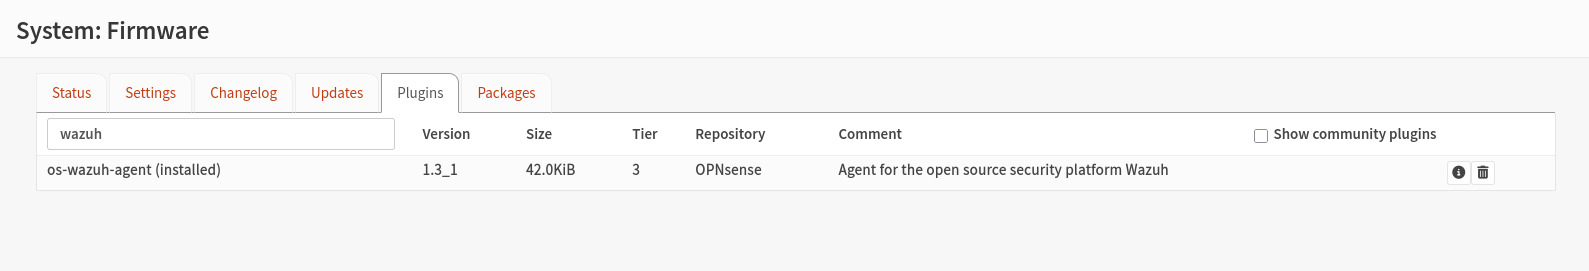
\includegraphics[scale=0.3]{tablas-images/pmv/fig27.jpeg}
	\caption{Plugin de Wazuh}\label{fig:fig27}
\end{figure}

\begin{figure}[H]
	\centering
	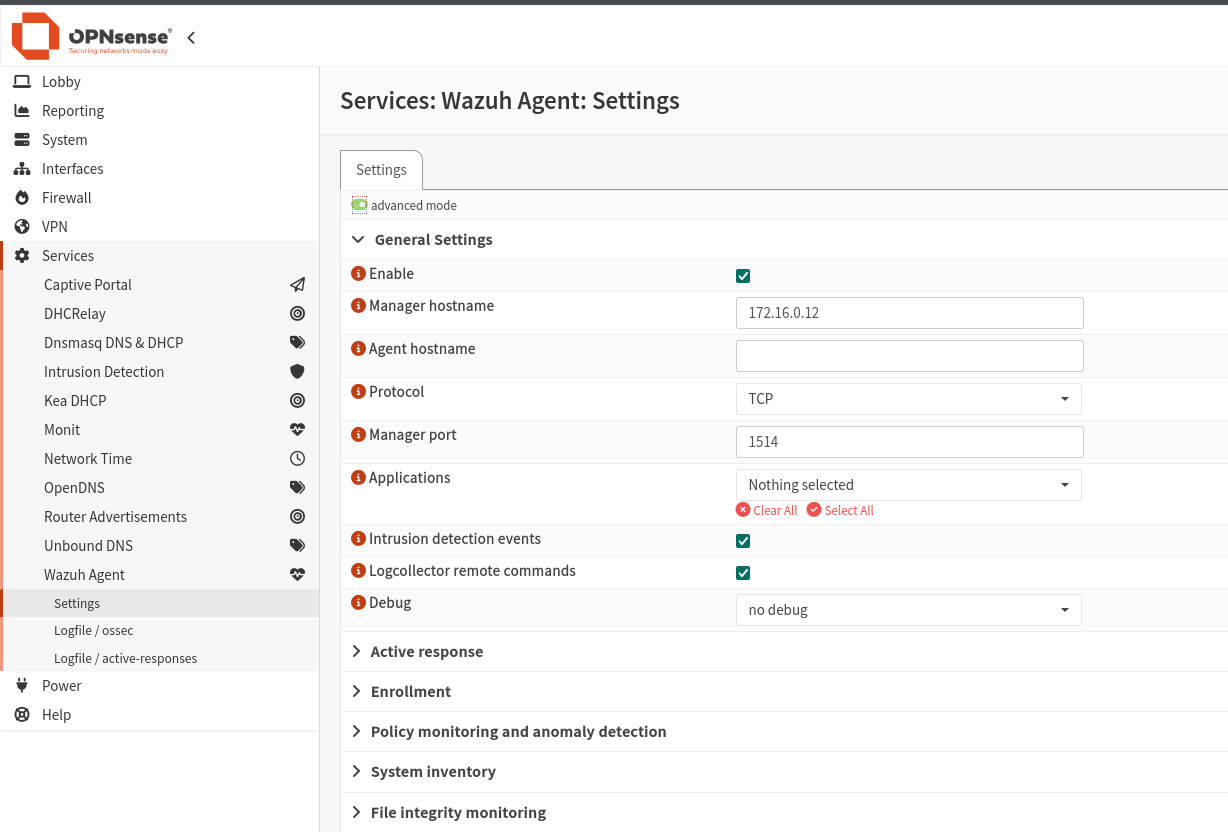
\includegraphics[scale=0.3]{tablas-images/pmv/fig28.jpeg}
	\caption{Configuración en OpnSense}\label{fig:fig28}
\end{figure}

En la máquina objetivo, al instalar el agente de Wazuh, se genera automáticamente una carpeta en la ruta previamente especificada, desde la 
cual es posible configurar el comportamiento del agente. Entre estas configuraciones se encuentra la definición del servidor al que serán 
enviados los registros, así como la especificación de los elementos, actividades y eventos que deben o no ser monitoreados y analizados 
antes de remitir la información al \textit{wazuh-manager}.

En la Figura~\ref{fig:fig29} se presenta la configuración realizada para el agente Wazuh desplegado en la máquina 
objetivo.

\begin{figure}[H]
	\centering
	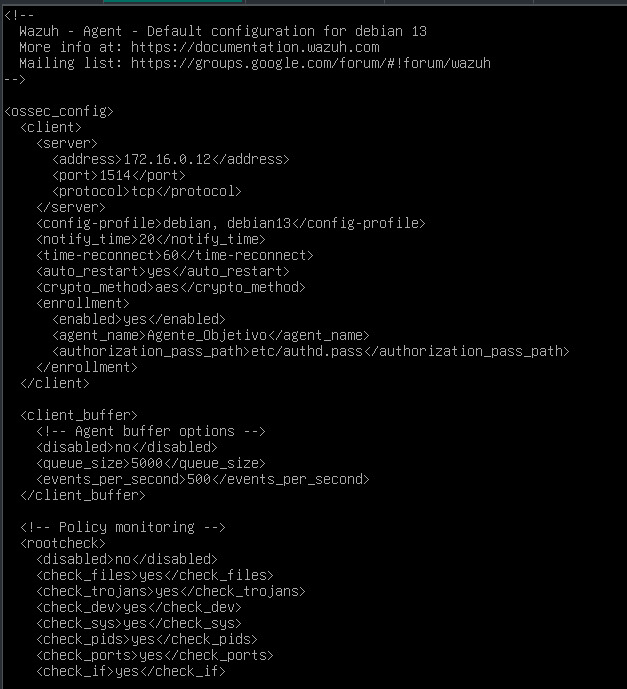
\includegraphics[scale=0.5]{tablas-images/pmv/fig29.jpeg}
	\caption{Archivo de configuración del agente de Wazuh en la máquina objetivo}\label{fig:fig29}
\end{figure}

Por su parte, Suricata, al desempeñar el rol de inspección y análisis del tráfico de red, genera registros y alertas cada vez que detecta 
actividades sospechosas, paquetes asociados a firmas maliciosas o descargas potencialmente perjudiciales para la infraestructura. Dichos 
eventos son almacenados principalmente en el archivo \texttt{eve.json}, considerado uno de los elementos más importantes para el 
diagnóstico y monitoreo continuo del entorno de seguridad.

Debido a la relevancia de esta información, se configura explícitamente el agente de Wazuh para que lea el contenido del archivo 
\texttt{eve.json} y envíe los registros al \textit{wazuh-manager}, permitiendo posteriormente realizar procesos de análisis, 
visualización y correlación de eventos de seguridad, evidencia que se muestra en la Figura~\ref{fig:fig30}.

Adicionalmente, no solo es necesario configurar el agente de Wazuh para monitorear este archivo, sino también ajustar el archivo 
\texttt{ossec.conf} del servidor Wazuh, con el fin de habilitar el procesamiento de registros en formato \texttt{JSON}. En la 
Figura~\ref{fig:fig31} se evidencia la configuración realizada en ambos archivos y el una segunda parte en la Figura~\ref{fig:fig32}.

\begin{figure}[H]
	\centering
	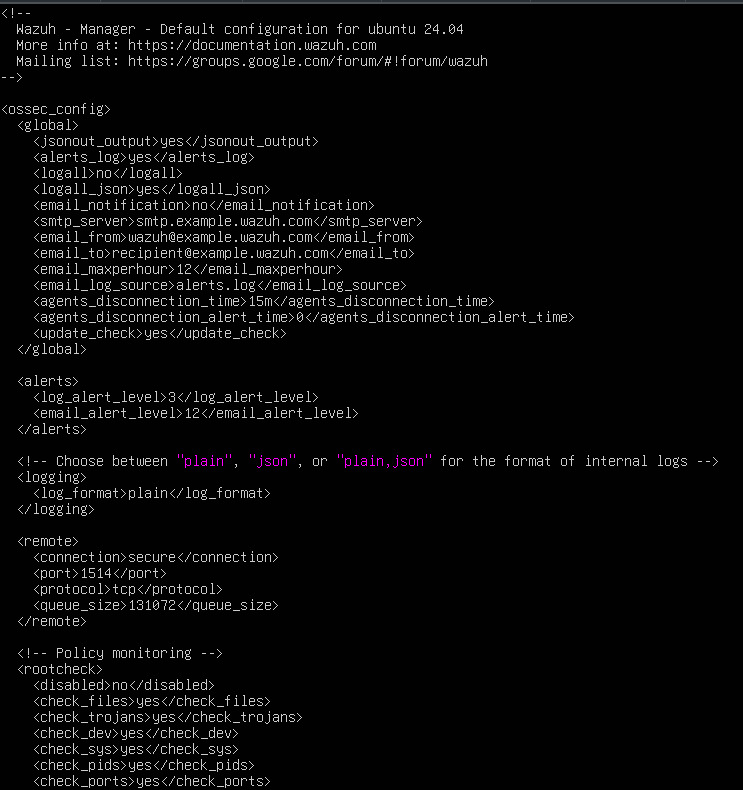
\includegraphics[scale=0.4]{tablas-images/pmv/fig30.jpeg}
	\caption{Configuración servidor Wazuh}\label{fig:fig30}
\end{figure}

\begin{figure}[H]
	\centering
	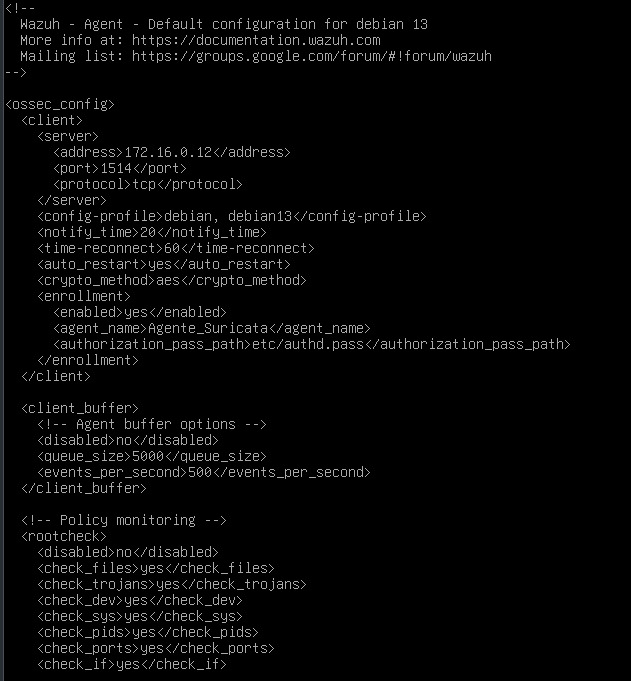
\includegraphics[scale=0.5]{tablas-images/pmv/fig31.jpeg}
	\caption{Configuración agente wazuh en suricata primera parte}\label{fig:fig31}
\end{figure}


\begin{figure}[H]
	\centering
	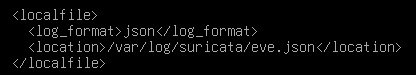
\includegraphics[scale=0.6]{tablas-images/pmv/fig32.jpeg}
	\caption{Configuración agente wazuh en suricata segunda parte}\label{fig:fig32}
\end{figure}

En el apartado de monitoreo, la herramienta SIEM Wazuh posee la capacidad de generar diferentes vistas e integrarlas dentro de su 
\textit{dashboard} principal, permitiendo visualizar de manera centralizada los registros de eventos generados tanto en las máquinas 
monitoreadas como en el tráfico de red analizado.

Para esta implementación, se desarrollaron cuatro vistas específicas con el objetivo de facilitar las tareas de análisis, supervisión y 
monitoreo de la infraestructura del laboratorio virtual. En la Figura~\ref{fig:fig33} se presentan las cuatro vistas 
configuradas en la plataforma.

\begin{figure}[H]
	\centering
	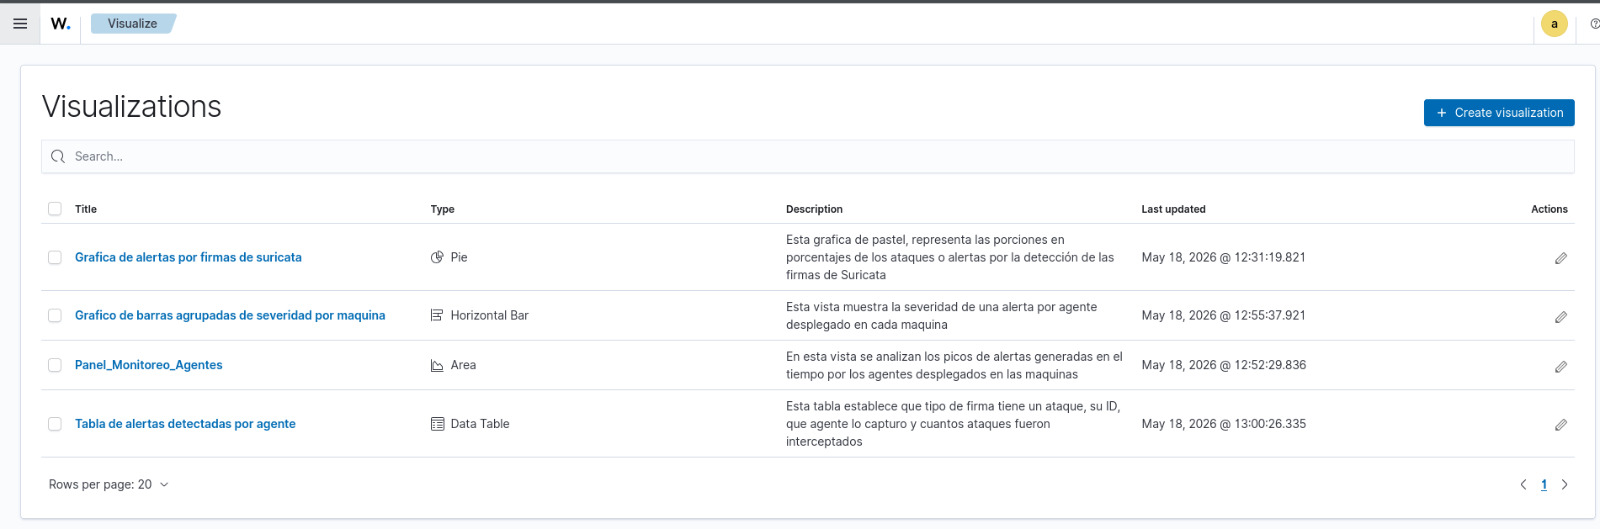
\includegraphics[scale=0.3]{tablas-images/pmv/fig33.jpeg}
	\caption{Lista de vistas  que componen el dashboard}\label{fig:fig33}
\end{figure}

Al describir cada una de las vistas implementadas, se inicia con la gráfica de alertas por firmas de Suricata. Esta corresponde a una 
gráfica de tipo pastel, en la cual se representa el porcentaje de alertas detectadas a partir de las reglas de firmas configuradas en 
Suricata. Dichas alertas son generadas mediante el análisis del tráfico de red, tanto del tránsito hacia Internet como de las 
comunicaciones internas entre los diferentes segmentos de red del laboratorio virtual.

En la Figura~\ref{fig:fig34} se presenta la gráfica correspondiente y su distribución según cada tipo de firma 
detectada.

\begin{figure}[H]
	\centering
	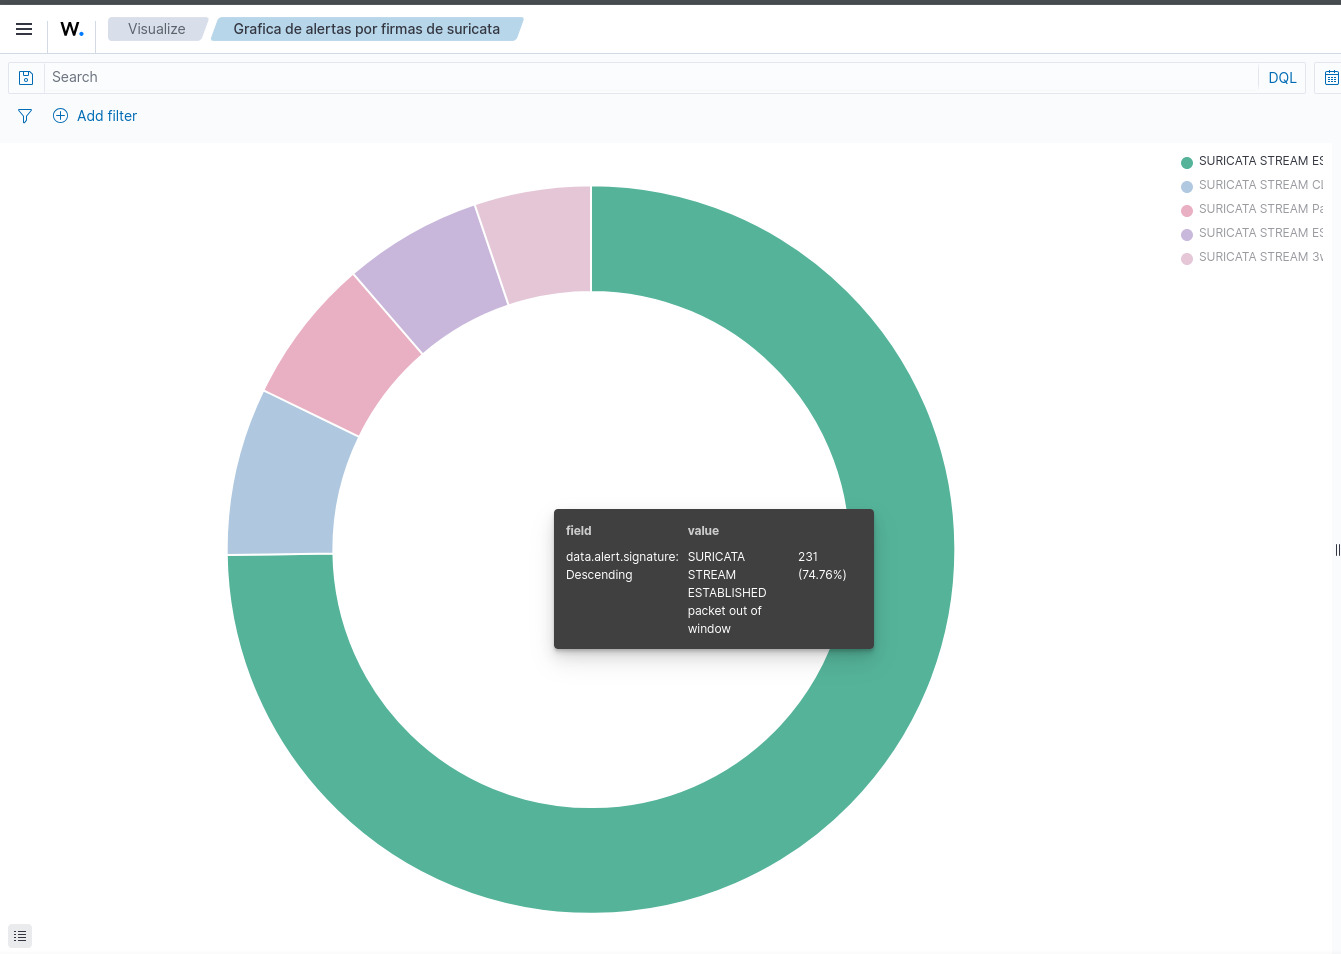
\includegraphics[scale=0.3]{tablas-images/pmv/fig34.jpeg}
	\caption{Vista de alertas por firma de suricata}\label{fig:fig34}
\end{figure}

La segunda vista, ilustrada en la Figura~\ref{fig:fig35}, corresponde a una gráfica de barras agrupadas cuya finalidad es 
representar los niveles de severidad asociados a las alertas generadas por el agente de la máquina donde ocurrió el evento. Esta 
visualización permite identificar de manera más clara la distribución y frecuencia de incidentes clasificados según su criticidad dentro 
de la infraestructura monitoreada.

\begin{figure}[H]
	\centering
	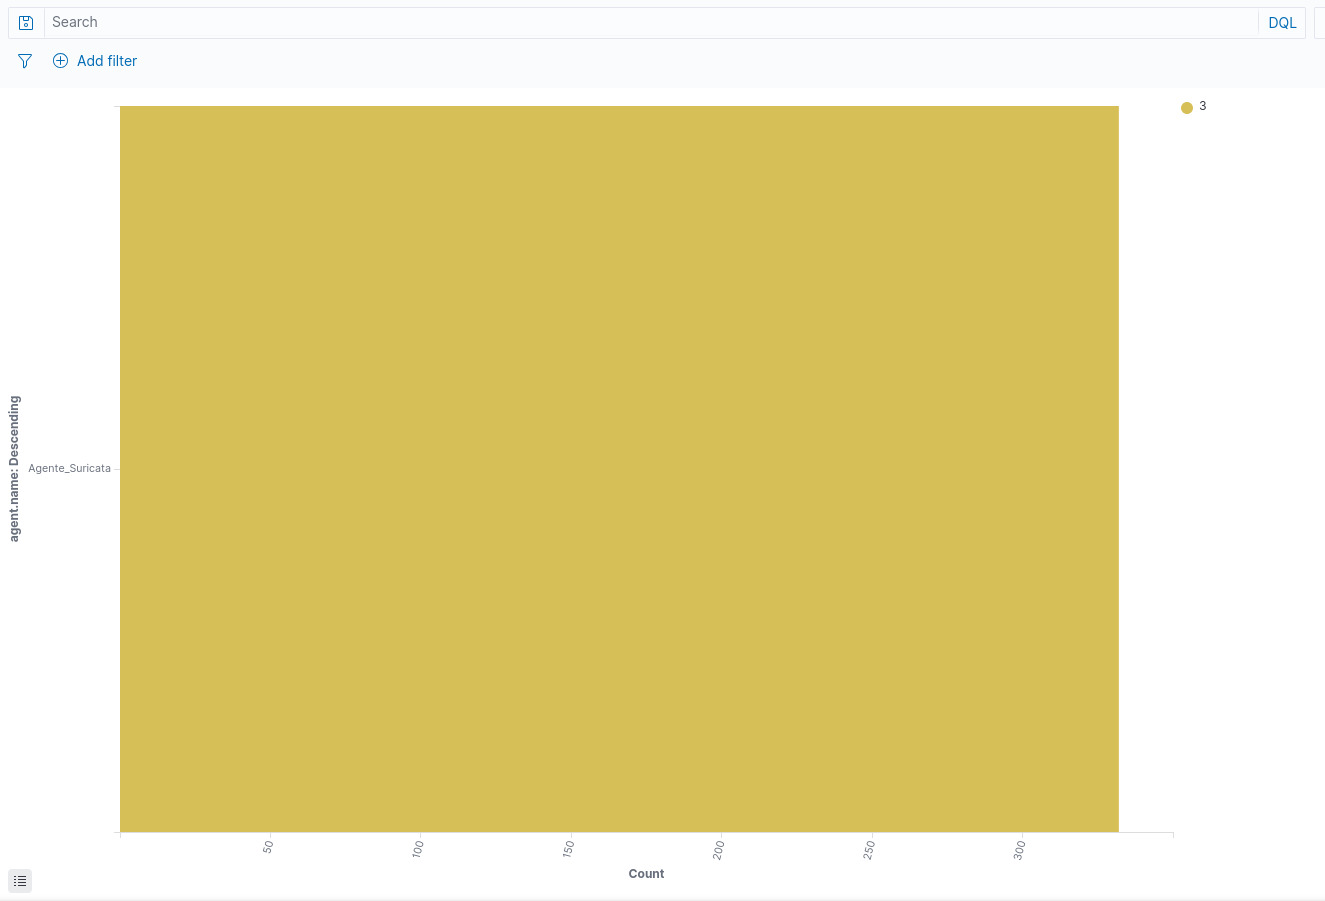
\includegraphics[scale=0.2]{tablas-images/pmv/fig35.jpeg}
	\caption{Vista de severidad de alerta por máquina}\label{fig:fig35}
\end{figure}

La tercera vista, presentada en la Figura~\ref{fig:fig36}, tiene como propósito mostrar la cantidad de alertas generadas por los agentes 
desplegados en cada máquina dentro de un intervalo de tiempo de 30 minutos. Este intervalo puede ser modificado según los requerimientos y 
necesidades de monitoreo establecidos por el cliente.

\begin{figure}[H]
	\centering
	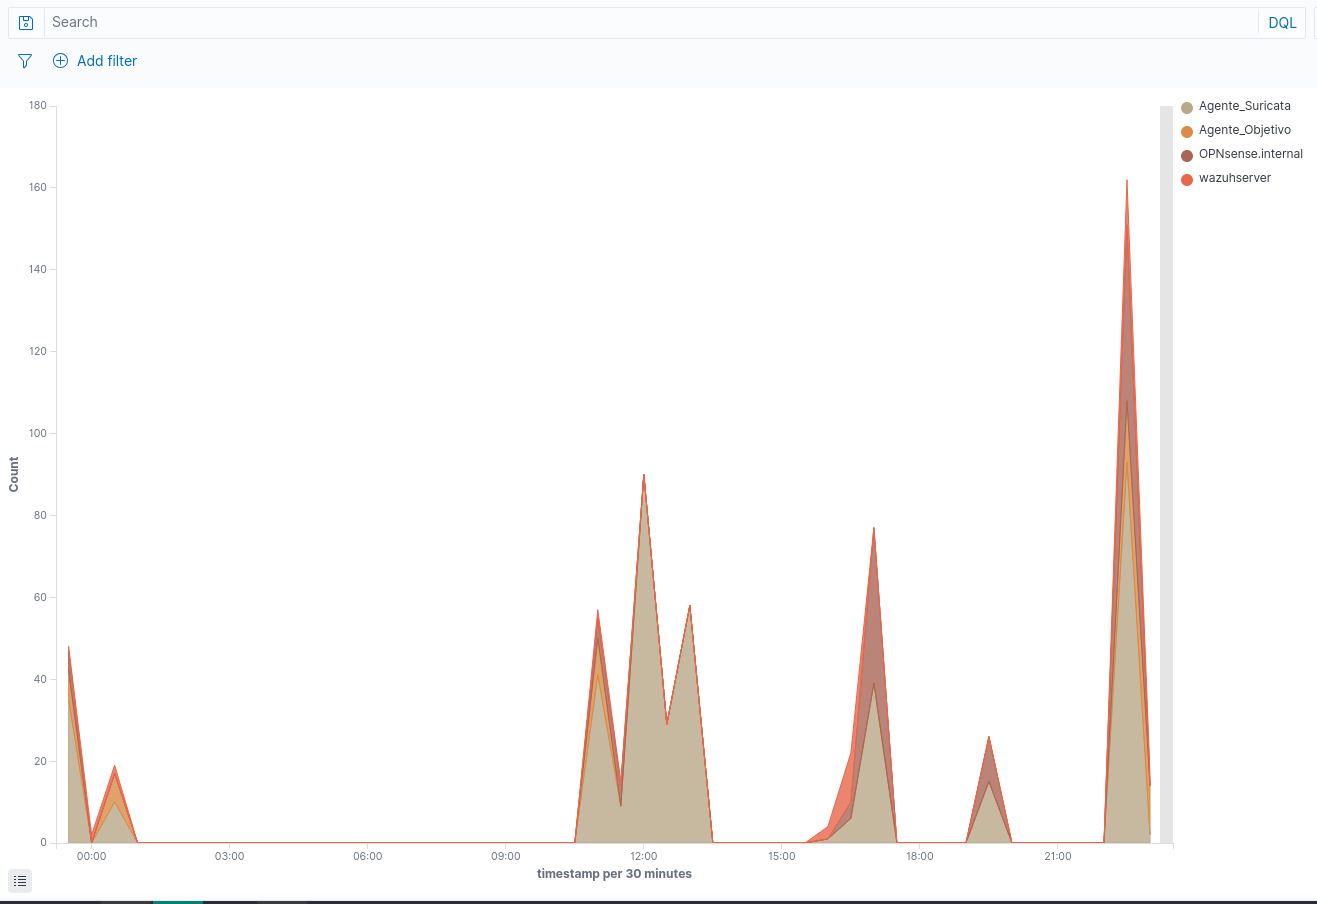
\includegraphics[scale=0.3]{tablas-images/pmv/fig36.jpeg}
	\caption{Vista de monitoreo de alertas por agente}\label{fig:fig36}
\end{figure}

Finalmente, en la Figura~\ref{fig:fig37} se presenta la tabla de alertas detectadas por los agentes desplegados en las diferentes máquinas 
de la infraestructura. Su función principal es exponer las alertas generadas a partir de las firmas detectadas por Suricata, incluyendo 
información relevante como el identificador de la alerta, el agente que reportó el evento y la cantidad de veces que dichas alertas fueron 
emitidas durante el monitoreo de la red.

\begin{figure}[H]
	\centering
	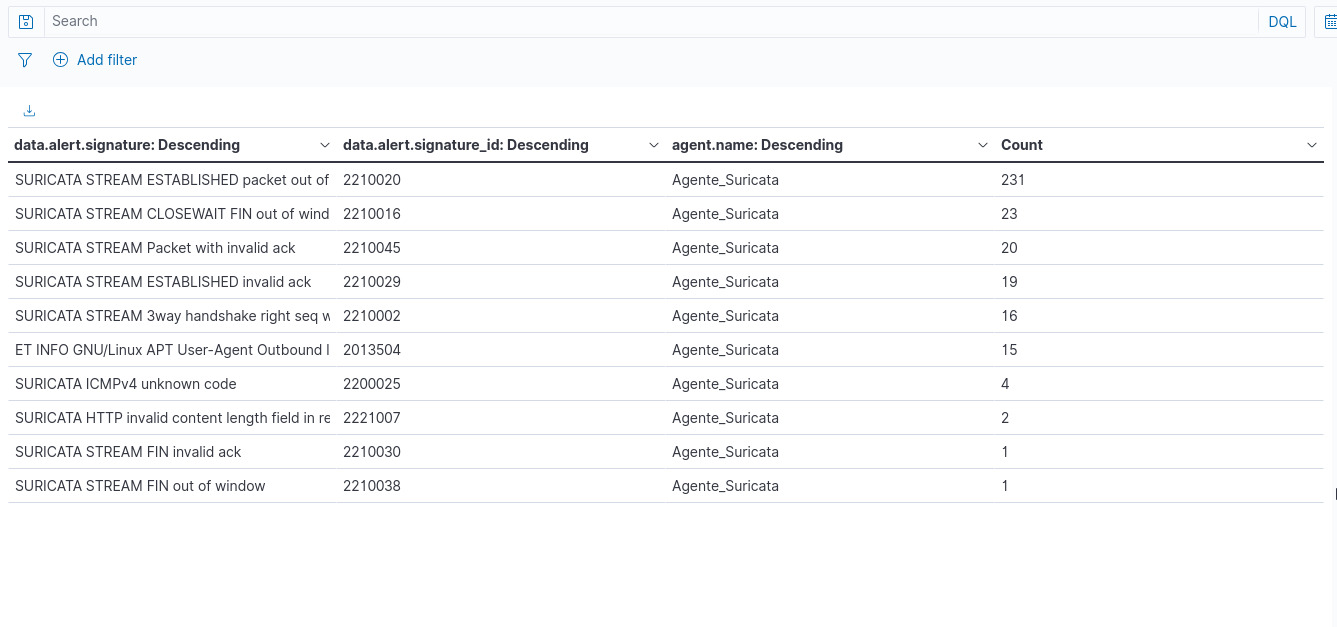
\includegraphics[scale=0.3]{tablas-images/pmv/fig37.jpeg}
	\caption{Vista de tabla de alertas por agente}\label{fig:fig37}
\end{figure}

Todas las vistas previamente descritas se integran en un \textit{dashboard} centralizado, cuya finalidad es facilitar las tareas de 
visualización, monitoreo y auditoría del tráfico de red, así como la gestión de eventos de seguridad dentro de la infraestructura del 
grupo GRID. En la Figura~\ref{fig:fig38} se presenta el \textit{dashboard} con las vistas integradas en la plataforma Wazuh.

\begin{figure}[H]
	\centering
	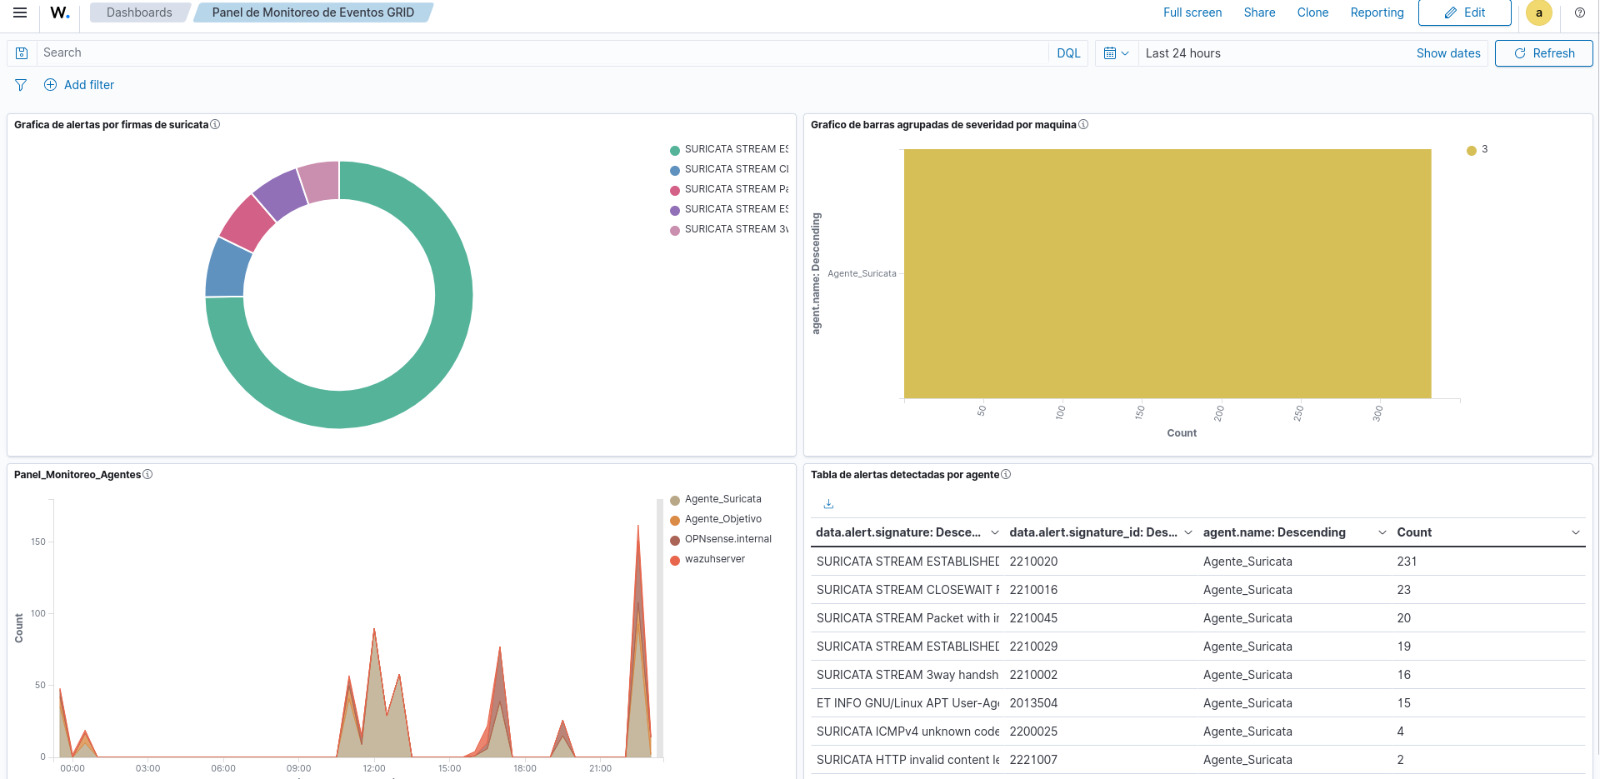
\includegraphics[scale=0.3]{tablas-images/pmv/fig38.jpeg}
	\caption{Panel de monitoreo de eventos GRID (Dashboard)}\label{fig:fig38}
\end{figure}

Es importante recalcar que este \textit{dashboard} fue personalizado de acuerdo con los requerimientos específicos de la infraestructura 
analizada. Sin embargo, la herramienta SIEM Wazuh también dispone de capacidades orientadas al cumplimiento y visualización de registros 
basados en estándares reconocidos de seguridad, como el NIST SP 800-53~\cite{NIST80053r5}.

En la Figura~\ref{fig:fig39} se presenta la visualización del \textit{dashboard} bajo este estándar de seguridad, 
permitiendo un enfoque orientado al monitoreo y gestión de controles de seguridad alineados con las directrices establecidas por el 
National Institute of Standards and Technology (NIST).

\begin{figure}[H]
	\centering
	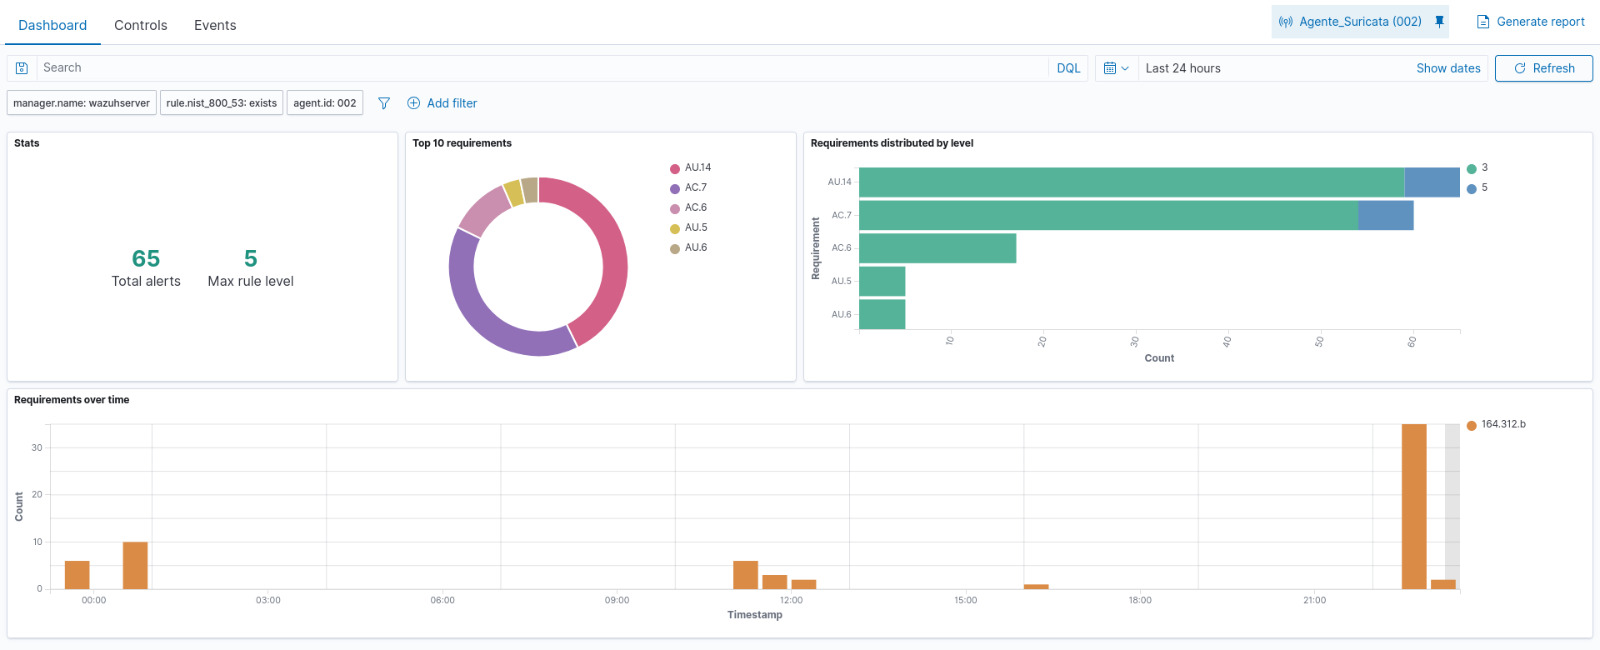
\includegraphics[scale=0.3]{tablas-images/pmv/fig39.jpeg}
	\caption{Dashboard bajo estándar NIST 800-53}\label{fig:fig39}
\end{figure}

Por último, se implementó el mecanismo de respuesta activa configurado desde la herramienta SIEM Wazuh hacia el firewall OpnSense, con el 
propósito de aplicar medidas de bloqueo sobre cualquier dirección IP que intente ejecutar o se encuentre realizando actividades maliciosas 
detectadas tanto por el agente de Wazuh como por el agente asociado a Suricata. En este punto se materializa la correlación de eventos, ya 
que Wazuh analiza las trazas y registros proporcionados por los agentes desplegados y, con base en las reglas y condiciones configuradas, 
toma decisiones automáticas orientadas a la mitigación de amenazas.

El primer paso consistió en configurar la comunicación entre Wazuh y OpnSense. Gracias al \textit{plugin} del agente Wazuh previamente 
instalado y configurado en OpnSense, se facilita la interacción entre ambas máquinas, siendo el servidor Wazuh quien emite las 
instrucciones mediante el agente desplegado en el firewall.

En la Figura~\ref{fig:fig40} se evidencia la configuración realizada para habilitar el proceso de respuesta activa del agente Wazuh. 
Asimismo, previamente se mencionó la regla de firewall ubicada en la interfaz WAN, cuyo origen corresponde al alias del agente 
\texttt{\_\_wazuh\_agent\_drop}. Esta configuración permite otorgar a Wazuh la capacidad de controlar y bloquear el tránsito de tráfico 
asociado a direcciones IP identificadas como potencialmente maliciosas.

\begin{figure}[H]
	\centering
	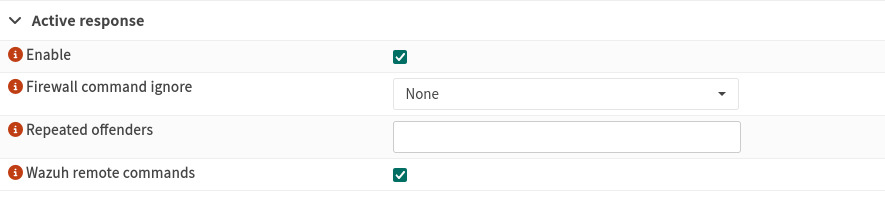
\includegraphics[scale=0.4]{tablas-images/pmv/fig40.jpeg}
	\caption{Habilitación y configuración de la respuesta activa}\label{fig:fig40}
\end{figure}

Posteriormente a la adecuación de la respuesta activa en el firewall, es necesario configurar el \textit{wazuh-manager} mediante el 
archivo \texttt{ossec.conf}, encargado de administrar y procesar todos los registros que ingresan y salen de la plataforma. En esta 
configuración se habilita el comando denominado \texttt{firewall-drop}, el cual permite que el agente de OpnSense identificado con el ID 
\texttt{001}, en conjunto con las reglas generadas por Suricata, emita la orden al firewall para bloquear direcciones IP sospechosas 
durante un tiempo estimado de 300 segundos.

Este mecanismo tiene como finalidad incluir temporalmente al atacante dentro de una lista negra alojada en la tabla de direcciones IP 
generada por el alias del agente Wazuh, la cual es interpretada por OpnSense para identificar las direcciones IP que deben ser bloqueadas 
automáticamente.

En la Figura~\ref{fig:fig41} se evidencia la configuración realizada en el archivo \texttt{ossec.conf} para habilitar 
la respuesta activa desde el \textit{wazuh-manager}. Asimismo, es importante recalcar que, una vez aplicada esta configuración, resulta 
indispensable reiniciar el servicio correspondiente para que los cambios surtan efecto correctamente.

\begin{figure}[H]
	\centering
	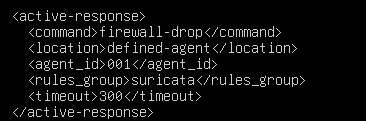
\includegraphics[scale=0.6]{tablas-images/pmv/fig41.jpeg}
	\caption{Configuración de respuesta activa en archivo ossec.conf}\label{fig:fig41}
\end{figure}

La implementación de la herramienta de código abierto SIEM Wazuh permitió el establecimiento de procesos de monitoreo continuo bajo el 
estándar NIST SP 800-53~\cite{NIST80053r5}, análisis forense, correlación de eventos y respuesta activa. Por consiguiente, se da 
cumplimiento práctico a los controles A.5.7, A.8.16, A.5.24 y A.5.31 de la ISO/IEC 27001:2022, así como a los controles CLD 12.4.1 y 
CLD 12.4.5 de la \ISO/IEC 27017:2015.

Finalmente, luego de implementar los aspectos de seguridad mediante una arquitectura de defensa en profundidad, así como de comprender 
cada una de las máquinas creadas, sus configuraciones, protocolos, conexiones, procesos de monitoreo continuo y mecanismos de respuesta 
activa, se presenta en la Figura 32 un diagrama que expone de forma gráfica la composición general del laboratorio virtual implementado.

\begin{figure}[H]
	\centering
	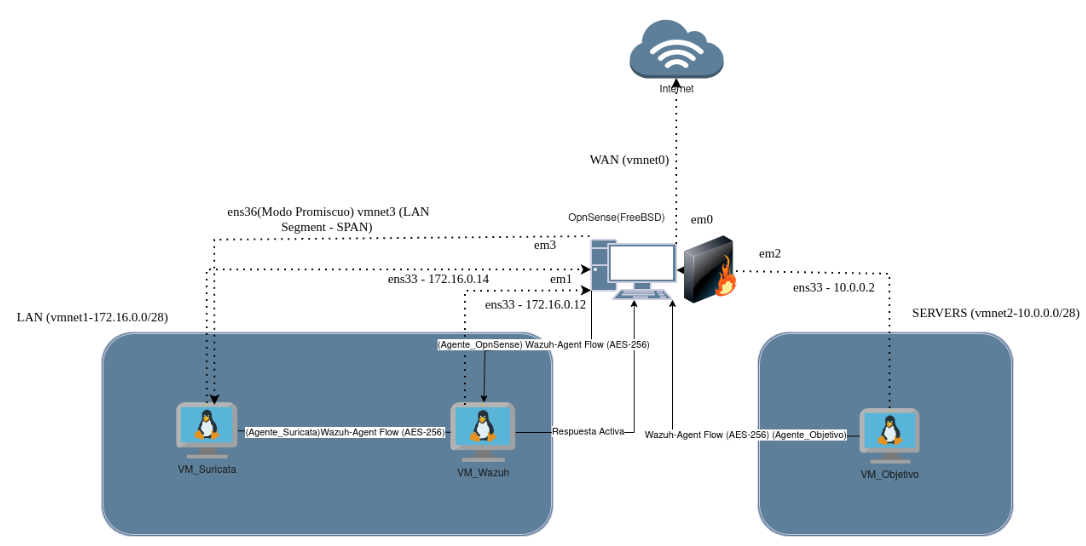
\includegraphics[scale=0.5]{tablas-images/pmv/fig42.png}
	\caption{Diagrama de topología de red final}\label{fig:fig42}
\end{figure}

\subsection{Conclusiones}
\noindent

La implementación de este laboratorio validó la efectividad de una arquitectura de Defensa en Profundidad mediante la integración de las 
herramientas de código abierto OPNsense, Suricata y Wazuh. El firewall perimetral garantizó el control de acceso y el aislamiento de los 
segmentos de red, mientras que el IDPS, configurado en modo promiscuo a través de la técnica de \textit{port mirroring}, permitió realizar 
una inspección profunda del tráfico sin degradar el rendimiento de los servidores. Toda esta telemetría de red se centralizó de forma 
transparente en el SIEM mediante el análisis estructurado del archivo \textit{eve.json}, eliminando los silos de información en la 
recolección de registros de eventos.

A nivel operativo, el proyecto permitió pasar de un esquema de monitoreo pasivo a un modelo de mitigación dinámica gracias a la 
funcionalidad de Respuesta Activa implementada en Wazuh. La integración entre Wazuh y OPNsense posibilitó que el sistema reaccionara de 
forma autónoma ante alertas críticas, aplicando directivas de bloqueo dinámico en el firewall para contener posibles ataques. Asimismo, el 
despliegue del firewall demostró que es viable homologar y simplificar la lógica de filtrado esencial previamente utilizada en herramientas
como Shorewall dentro de interfaces de estado modernas, permitiendo establecer capacidades de monitoreo continuo, manteniendo un entorno 
seguro, organizado y fácil de auditar.

Finalmente, el entorno virtualizado funcionó como un escenario práctico para materializar los requerimientos de gobernanza y seguridad del 
Grupo GRID en configuraciones técnicas reales. El diseño del laboratorio, el análisis de amenazas basado en firmas globales y la 
centralización de eventos de seguridad permitieron dar cumplimiento técnico y demostrable a los controles A.5.7, A.5.24, A.5.31, A.8.16, 
A.8.6 y A.8.22 de la norma ISO/IEC 27001:2022, así como a los controles CLD 12.4.1 y CLD 12.4.5 de la ISO/IEC 27017:2015, consolidando una 
infraestructura alineada con estándares internacionales de seguridad de la información.

